\documentclass[nobib]{tufte-handout}

%\\geometry{showframe}% for debugging purposes -- displays the margins

\newcommand{\bra}[1]{\left(#1\right)}
\usepackage{amssymb}
\usepackage{hyperref}
\usepackage[activate={true,nocompatibility},final,tracking=true,kerning=true,spacing=true,factor=1100,stretch=10,shrink=10]{microtype}
\usepackage{color}
\usepackage{steinmetz}
% Fixes captions and images being cut off
\usepackage{marginfix}
\usepackage{array}
\usepackage{tikz}
\usepackage{pgfplots}
\usepackage{amsmath,amsthm}
\usetikzlibrary{shapes}
\usetikzlibrary{positioning}
\usepackage{listings}
\usepackage{caption}
\usepackage[americancurrents, americanvoltages, americanresistors, americaninductors]{circuitikz}
\DeclareCaptionFont{white}{\color{white}}
\DeclareCaptionFormat{listing}{\colorbox{gray}{\parbox{\textwidth}{#1#2#3}}}
\captionsetup[lstlisting]{format=listing,labelfont=white,textfont=white}

% Set up the images/graphics package
\usepackage{graphicx}
\setkeys{Gin}{width=\linewidth,totalheight=\textheight,keepaspectratio}
\graphicspath{{.}}

\title{ECE 20002: Electrical Engineering Fundamentals II}
\author[Zeke Ulrich]{Zeke Ulrich}
\date{\today}  % if the \date{} command is left out, the current date will be used

% The following package makes prettier tables.  We're all about the bling!
\usepackage{booktabs}

% The units package provides nice, non-stacked fractions and better spacing
% for units.
\usepackage{units}

% The fancyvrb package lets us customize the formatting of verbatim
% environments.  We use a slightly smaller font.
\usepackage{fancyvrb}
\fvset{fontsize=\normalsize}

% Small sections of multiple columns
\usepackage{multicol}

% For finite state machines 
\usetikzlibrary{automata} % Import library for drawing automata
\usetikzlibrary{positioning} % ...positioning nodes
\usetikzlibrary{arrows} % ...customizing arrows
\tikzset{node distance=2.5cm, % Minimum distance between two nodes. Change if necessary.
    every state/.style={ % Sets the properties for each state
    semithick,
    fill=gray!10},
    initial text={}, % No label on start arrow
    double distance=2pt, % Adjust appearance of accept states
    every edge/.style={ % Sets the properties for each transition
    draw,
    ->,>=stealth', % Makes edges directed with bold arrowheads
    auto,
    semithick}}
\let\epsilon\varepsilon

% These commands are used to pretty-print LaTeX commands
\newcommand{\doccmd}[1]{\texttt{\textbackslash#1}}% command name -- adds backslash automatically
\newcommand{\docopt}[1]{\ensuremath{\langle}\textrm{\textit{#1}}\ensuremath{\rangle}}% optional command argument
\newcommand{\docarg}[1]{\textrm{\textit{#1}}}% (required) command argument
\newenvironment{docspec}{\begin{quote}\noindent}{\end{quote}}% command specification environment
\newcommand{\docenv}[1]{\textsf{#1}}% environment name
\newcommand{\docpkg}[1]{\texttt{#1}}% package name
\newcommand{\doccls}[1]{\texttt{#1}}% document class name
\newcommand{\docclsopt}[1]{\texttt{#1}}% document class option name

% Define a custom command for definitions and biconditional
\newcommand{\defn}[2]{\noindent\textbf{#1}:\ #2}
\let\biconditional\leftrightarrow

% Define graphics path
\graphicspath{ {./images/} }

\tikzset{
  mirror/.code={
    \def\mirrortemp{#1} % Store the content to be mirrored
    \begin{scope}[xscale=-1] % Mirror horizontally
      \path \mirrortemp; % Draw the mirrored path
    \end{scope}
  }
}

\begin{document}

\maketitle

\begin{abstract}
    Lecture notes for Purdue's ECE 20002.
\end{abstract}

\tableofcontents

\section{Course Introduction}

Continuation of Electrical Engineering Fundamentals I. The course addresses
mathematical and computational foundations of circuit analysis (differential
equations, Laplace Transform techniques) with a focus on application to linear
circuits having variable behavior as a function of frequency, with emphasis on
filtering. Variable frequency behavior is considered for applications of
electronic components through single-transistor and operational amplifiers. The
course ends with a consideration of how circuits behave and may be modeled for
analysis at high frequencies.\\~\\ Learning Objectives:
\begin{enumerate}
    \item Analyze 2nd order linear circuits with sources and/or passive elements
    \item Compute responses of linear circuits with and without initial conditions via
          one-sided Laplace transform techniques
    \item Compute responses to linear circuits using transfer function and convolution
          techniques
    \item Analyze and design transistor amplifiers at low, mid and high frequencies
\end{enumerate}

\pagebreak

\section{Field-Effect Transistor Devices}

\subsection{MOSFETs}
Let us begin where ECE 20001 ended, with metal-oxide semiconductor 
field-effect transistors (MOSFETs). The rectangle below represent 
a wafer of silicon. The p - Si label indicates that the 
the wafer is primarily doped with boron and the primary carrier
type is holes. The two $n^+$ rectangles designate regions of phosphorus 
doping. The grey rectangles above the wafer are dielectric layers of 
silicon dioxide. The black rectangles are ohmic metals 
that allow for connecting our phosphorus regions to other components.
To these metal contacts we attach a source, a gate, and a drain.  
The source is the source of electron, and the drain is how the electrons 
exit. The gate will define a pathway between the source and drain. 
\begin{figure}
    \caption{nMOSFET diagram}
    \label{fig:nMOSFET diagram}
    \begin{center}
        \begin{circuitikz}
            \draw (0,0)
            to (4,0)
            to (4,2)
            to (0,2)
            to (0,0);
            \node at (2,1) {p - Si};
            \draw (2,0) to (2,-0.25) node[ground]{};
    
            \draw (0.5, 2) rectangle node {$n^+$} (1.5,1.5);
            \draw (2.5, 2) rectangle node {$n^+$} (3.5,1.5);
    
            \draw[fill=gray] (0,2) rectangle (0.5,2.25);
            \draw[fill=gray] (1.5,2) rectangle (2.5,2.25);
            \draw[fill=gray] (3.5,2) rectangle (4,2.25);
            
            \draw[fill=black] (0.5, 2) rectangle (1.5,2.125);
            \draw[fill=black] (1.5,2.25) rectangle (2.5,2.375);
            \draw[fill=black] (2.5, 2) rectangle (3.5,2.125);
    
            \draw (1, 2) to[short, -*] (1, 3) node[above] {Source}
            to (0.5, 3);
            \draw (2, 2.25) to[short, -*] (2, 3.25) node[above] {Gate, $v_{GS}(v_G)$};
            \draw (3, 2) to[short, -*] (3, 3) node[right] {Drain, $v_{DS}(v_D)$};
        \end{circuitikz}
    \end{center}
\end{figure}
Since the phosphorus regions are n-type and 
ergo have free electrons, the primary carrier of this MOSFET are electrons. 
The way we allow current to flow from source 
to drain is by increasing the voltage of the gate $v_{GS}$ to attract 
an inversion layer underneath the dielectric separating the gate from the 
silicon wafer. If the voltage of the gate is high enough ($v_{GS} > V_T$) then 
enough electrons will be attracted to that area for current to flow between 
source and drain. 

We could create a similar MOSFET by inverting the n-type and 
p-type regions, as in figure \ref{fig:pMOSFET}.
\begin{figure}
    \caption{pMOSFET diagram}
    \label{fig:pMOSFET}
    \begin{center}
        \begin{circuitikz}
            \draw (0,0)
            to (4,0)
            to (4,2)
            to (0,2)
            to (0,0);
            \node at (2,1) {n - Si};
            \draw (2,0) to (2,-0.25) node[ground]{};
    
            \draw (0.5, 2) rectangle node {$p^+$} (1.5,1.5);
            \draw (2.5, 2) rectangle node {$p^+$} (3.5,1.5);
    
            \draw[fill=gray] (0,2) rectangle (0.5,2.25);
            \draw[fill=gray] (1.5,2) rectangle (2.5,2.25);
            \draw[fill=gray] (3.5,2) rectangle (4,2.25);
            
            \draw[fill=black] (0.5, 2) rectangle (1.5,2.125);
            \draw[fill=black] (1.5,2.25) rectangle (2.5,2.375);
            \draw[fill=black] (2.5, 2) rectangle (3.5,2.125);
    
            \draw (1, 2) to[short, -*] (1, 3) node[above] {Source}
            to (0.5, 3);
            \draw (2, 2.25) to[short, -*] (2, 3.25) node[above] {Gate, $v_{GS}(v_G)$};
            \draw (3, 2) to[short, -*] (3, 3) node[right] {Drain, $v_{DS}(v_D)$};
        \end{circuitikz}
    \end{center}
\end{figure}
In this case the primary current carrier will be holes. 

In the case of the nMOSFET in figure \ref{fig:nMOSFET diagram}, 
a negative gate voltage will attract holes in the 
semiconductor, forming two oppositely charged areas separated 
by a distance $x$. This establishes an electric field 
within the oxide layer given by the equation for a 
parallel plate capacitor
\begin{equation} \label{eq:1}
    \mathcal{E}_x = - \frac{dV}{dx}
\end{equation}
Likewise, a positive gate voltage \emph{that is less than $V_T$} will attract electrons in the 
semiconductor. This also forms a capacitance of $C_{ox}$ in the
oxide layer, but because the semiconductor is n-type, the electrons will 
be spread out over a wider area and have their own capacitance $C_d$. 
Thus the total capacitance across the oxide and depletion region
$C$ given by
\begin{equation} \label{eq:2}
    \frac{1}{C} = \frac{1}{C_ox} + \frac{1}{C_d}
\end{equation}
If $0 < V_T < v_{GS}$, then $C=f{\omega}$, where $\omega$ is 
the frequency of our probe. 

Figure \ref{fig:p-type MOS C-V} displays the 
capacitance-voltage graph of a p-type metal-oxide 
semiconductor. The capacitance is constant when 
gate voltage is negative, then falls at the \emph{flat-band voltage}
$V_{GS} = 0V$, then rapidly rises again after the threshold voltage 
is reached. 
\begin{figure}
    \caption{p-type MOS capacitance-voltage characteristic}
    \label{fig:p-type MOS C-V}
    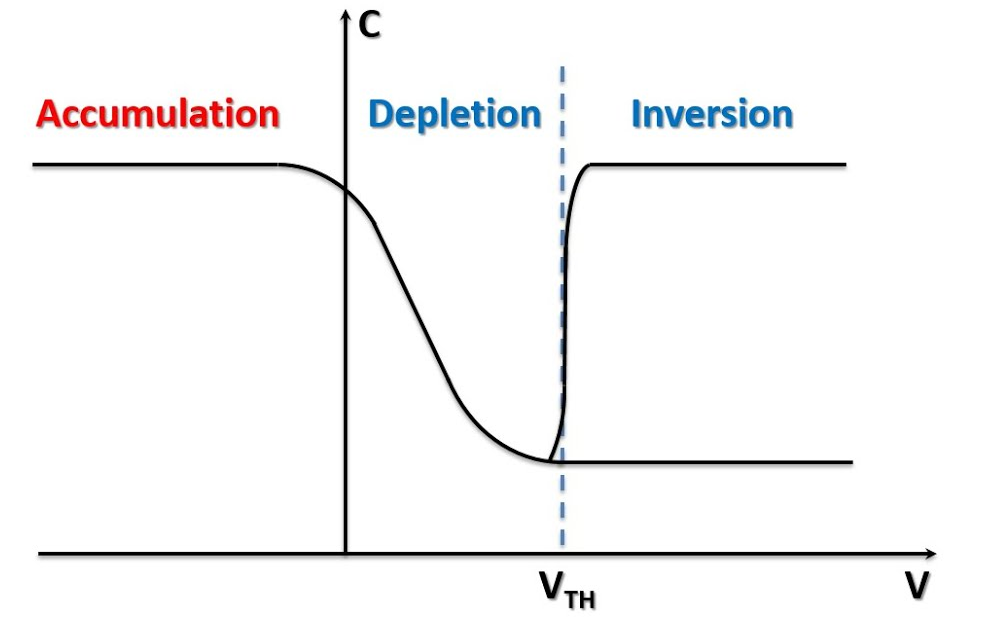
\includegraphics{moscv.png}
\end{figure}

The resistivity of the inversion channel created by the gate's bias
is given by 
\begin{equation} \label{eq:3}
    \frac{1}{\rho} = (n\mu_e + p\mu_h)q
\end{equation}
where $n$ is the concentration of electrons, 
$p$ is the concentration of holes, $\mu_e$ is
the mobility of electrons, $\mu_h$ is the 
mobility of holes, and $q$ is the charge of an electron. 
The higher the gate voltage, the higher the current between source and drain. 
Below the threshold voltage there is no current flow because no 
channel is formed. This relationship is linear provided the drain voltage 
is less than 150 mV, but above 0.3 V becomes nonlinear. That's because 
the channel is no longer a regular shape, but narrows in the region of the 
drain. Below 150 mV, however, this distortion can be assumed negligible. 
Recall that 
\begin{equation} \label{4}
    R = \frac{\rho L}{A}
\end{equation}
Whereas for small $v_{DS}$ the area is almost constant, 
when $v_{DS} > 0.15 V$ the area $A$ decreases enough that 
the resistance $R$ is significantly increased. When the area has 
decreased to zero at the drain, we reach the \emph{pinch-off} and 
the drain voltage is at saturation $v_{DS(sat)}$. The current still 
flows constantly for all drain voltage above saturation, however. 
Before saturation is reached and after the gate voltage is above the threshold, 
we are in the triode region. In the triode region, the current is given by 
\begin{equation} \label{eq:5}
    i_{D(triode)} = \mu C_{ox} \frac{W}{L} ((v_{GS}-V_T)v_{DS}-\frac{v^2_{DS}}{2})
\end{equation}
Sometimes, the constant terms are wrapped up into 
one constant, like so:
\begin{equation} \label{eq:6}
    i_{D(triode)} = k_n ((v_{GS}-V_T)v_{DS}-\frac{v^2_{DS}}{2})
\end{equation}
In the saturation region, 
\begin{align} \label{eq:7}
    i_{D(sat)} &= \mu C_{ox} \frac{W}{L} \frac{(v_{GS}-V_T)^2}{2} \\
    &= k_n \frac{v^2_{DS(sat)}}{2}
\end{align}
When we are far away from saturation, 
the resistance of the channel is given by 
\begin{align} \label{eq:8}
    R_{on} &= \frac{\partial v_{DS}}{\partial i_D} \\
    &= \frac{1}{\mu C_{ox} \frac{W}{L} (v_{GS} - V_T)}
\end{align}

Figure \ref{fig:Transfer Characteristics} shows a family of $i_D$-$v_{DS}$
curves with differing values of $v_{GS}$. 
\begin{figure}
    \caption{Transfer characteristics of nMOSFETs}
    \label{fig:Transfer Characteristics}
    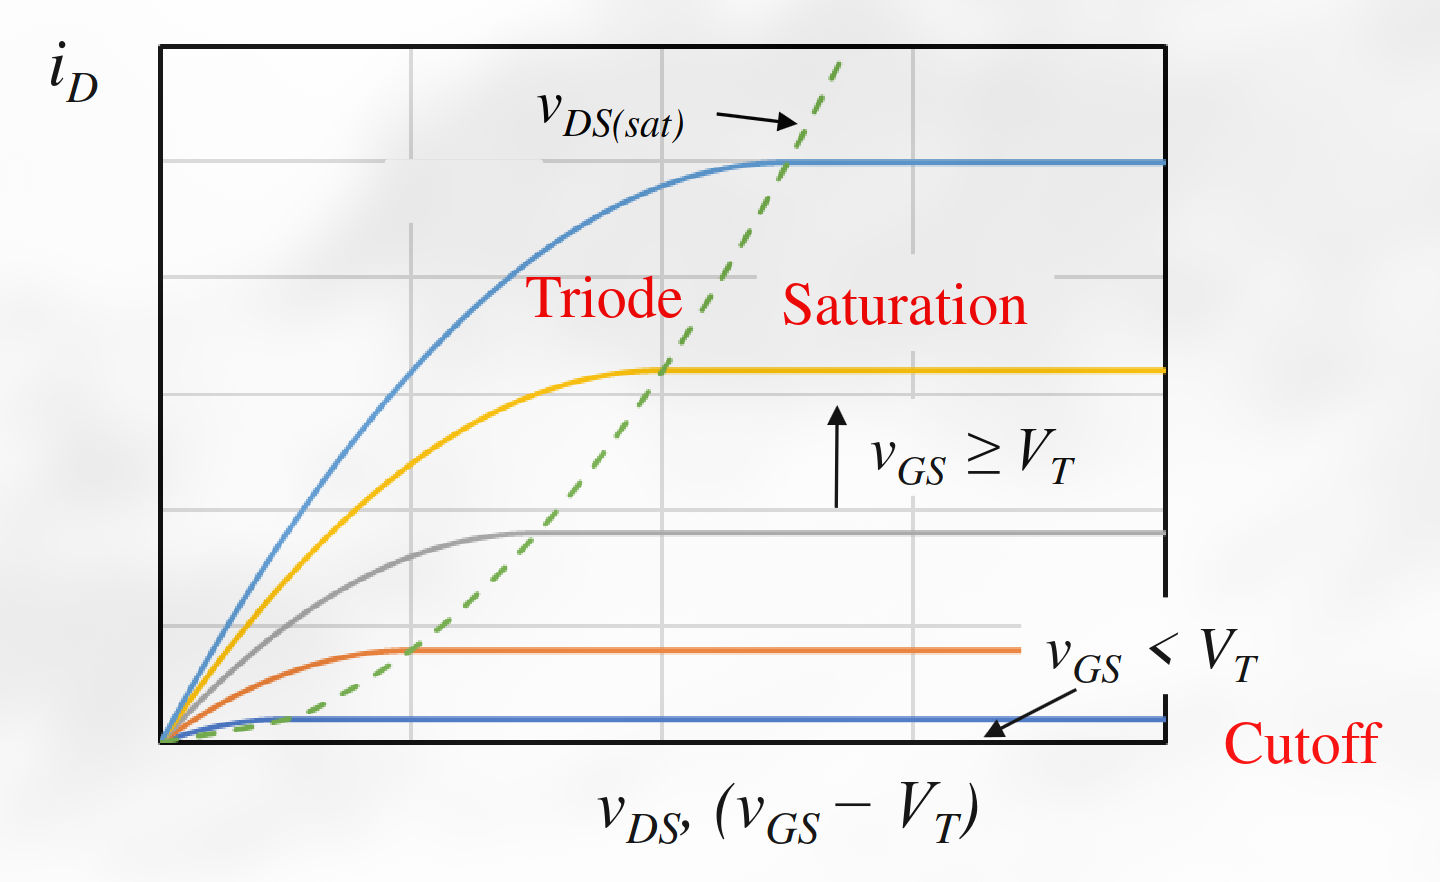
\includegraphics{Transfer Characteristics.png}
\end{figure}
Also show as a dashed green line is the saturation current 
as a function of gate voltage. Let's look at the impact 
the threshold voltage has by plotting the $i_D$-$v_{GS}$ curve 
for differing values of $V_T$ in figure \ref{fig:idvgsvt}. 
\begin{figure}
    \caption{$i_D$-$v_{GS}$ curve for select values of $V_T$}
    \label{fig:idvgsvt}
    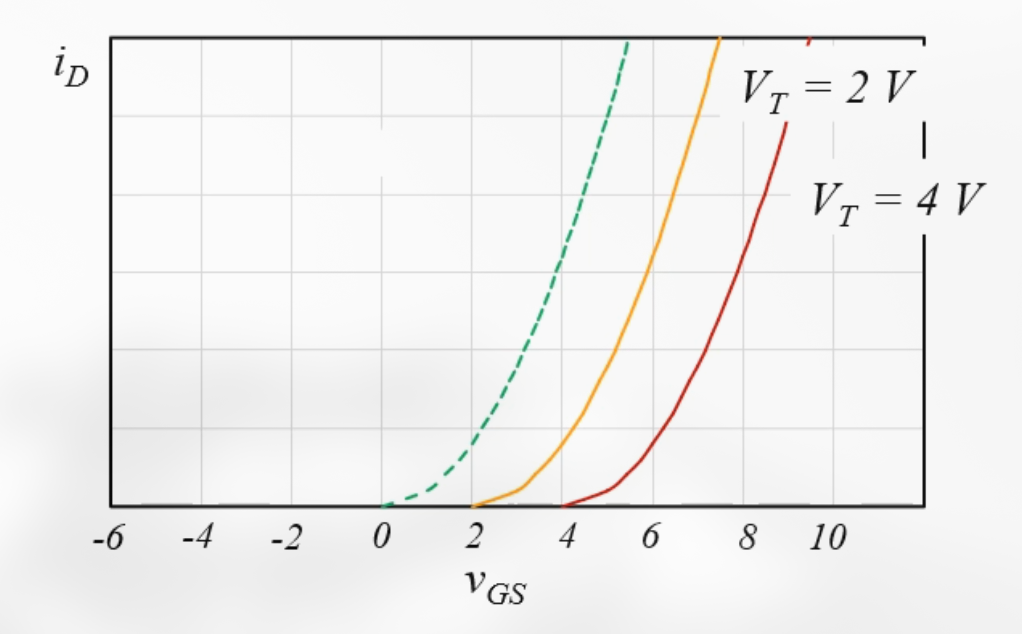
\includegraphics{idvgsvt.png}
\end{figure}
Now the green dashed curve corresponds to a threshold voltage of zero. 
Recall that the threshold voltage is intrinsic to 
the semiconductor wafer. Doping variations, defect, and shape can 
all affect the threshold voltage. If we build a depletion-mode nMOSFET,
then we allow for negative threshold voltages.

A normally off like in figure \ref{fig:nMOSFET diagram} 
has the symbol shown in \ref{fig:nMOSFET schematic} and 
is said to be in enhancement mode. 
\begin{figure}
    \caption{nMOSFET schematic}
    \label{fig:nMOSFET schematic}
    \begin{center}
        \begin{circuitikz}
            \draw (0,0) node[nmos] (mosfet) {};
            \draw (mosfet.D) -- ++(0,-0.5) node[right] {$V_{D}$};
            \draw (mosfet.S) -- ++(0,-0.1) node[right] {$V_S$}
            -- ++(0, 0.6) 
            -- ++(-0.5,0)
            to[short, i=~] ++(0.5,0);
            \draw (mosfet.G) -- ++(-0.5,0) node[left] {$V_{GS}$};
        \end{circuitikz}
    \end{center}
\end{figure}
If the nMOSFET has an n-channel between the source and 
drain, as shown in figure \ref{fig:nMOSFET diagram on}, 
\begin{figure}
    \caption{ Normally on nMOSFET diagram}
    \label{fig:nMOSFET diagram on}
    \begin{center}
        \begin{circuitikz}
            \draw (0,0)
            to (4,0)
            to (4,2)
            to (0,2)
            to (0,0);
            \node at (2,1) {p - Si};
            \draw (2,0) to (2,-0.25) node[ground]{};
    
            \draw (0.5, 2) rectangle node {$n^+$} (1.5,1.65);
            \draw (2.5, 2) rectangle node {$n^+$} (3.5,1.65);
    
            \draw[fill=gray] (0,2) rectangle (0.5,2.25);
            \draw[fill=gray] (1.5,2) rectangle (2.5,2.25);
            \draw[fill=gray] (3.5,2) rectangle (4,2.25);
            
            \draw[fill=black] (0.5, 2) rectangle (1.5,2.125);
            \draw[fill=black] (1.5,2.25) rectangle (2.5,2.375);
            \draw[fill=black] (2.5, 2) rectangle (3.5,2.125);
    
            \draw (1, 2) to[short, -*] (1, 3) node[above] {Source}
            to (0.5, 3);
            \draw (2, 2.25) to[short, -*] (2, 3.25) node[above] {Gate, $v_{GS}(v_G)$};
            \draw (3, 2) to[short, -*] (3, 3) node[right] {Drain, $v_{DS}(v_D)$};

            \draw[fill=green] (1.5, 2) rectangle (2.5, 1.75) node[below] {n-channel}; 
        \end{circuitikz}
    \end{center}
\end{figure}
then it is normally on and its symbol is as seen in 
figure \ref{fig:nMOSFET on schematic}. This kind of nMOSFET 
is said to be in depletion mode. 
\begin{figure}
    \caption{Schematic of normally on nMOSFET}
    \label{fig:nMOSFET on schematic}
    \begin{center}
        \begin{circuitikz}
            \draw (0,0) node[nmosd] (mosfet) {};
            \draw (mosfet.D) -- ++(0,-0.5) node[right] {$V_{D}$};
            \draw (mosfet.S) -- ++(0,-0.1) node[right] {$V_S$}
            -- ++(0, 0.6) 
            -- ++(-0.5,0)
            to[short, i=~] ++(0.5,0);
            \draw (mosfet.G) -- ++(-0.5,0) node[left] {$V_{GS}$};
        \end{circuitikz}
    \end{center}
\end{figure}
Note the thicker line between source and drain representing 
the n-channel. 

Similarly, the pMOSFET shown in figure \ref{fig:pMOSFET} is 
a normally off, enhancement mode pMOSFET. A pMOSFET with a 
p-channel is normally on and in depletion mode. 

Let's look at the transfer characteristics of 
the different types of MOSFETs. figure \ref{fig:Transfer Characteristics} 
shows these characteristics for a normally off, enhancement mode 
nMOSFET.
For a normally on, depletion mode nMOSFET the graph is exactly 
the same, except that the current can flow even when the 
gate bias is zero since the fabricated channel allows 
the flow of electrons from source to drain.
The output characteristics for a normally off, enhancement mode pMOSFET
are shown in figure \ref{fig:idvgsvt pmosfet}.
\begin{figure}
    \caption{$i_D$-$v_{DS}$ curve for select values of $v_{GS}-V_T$}
    \label{fig:idvgsvt pmosfet}
    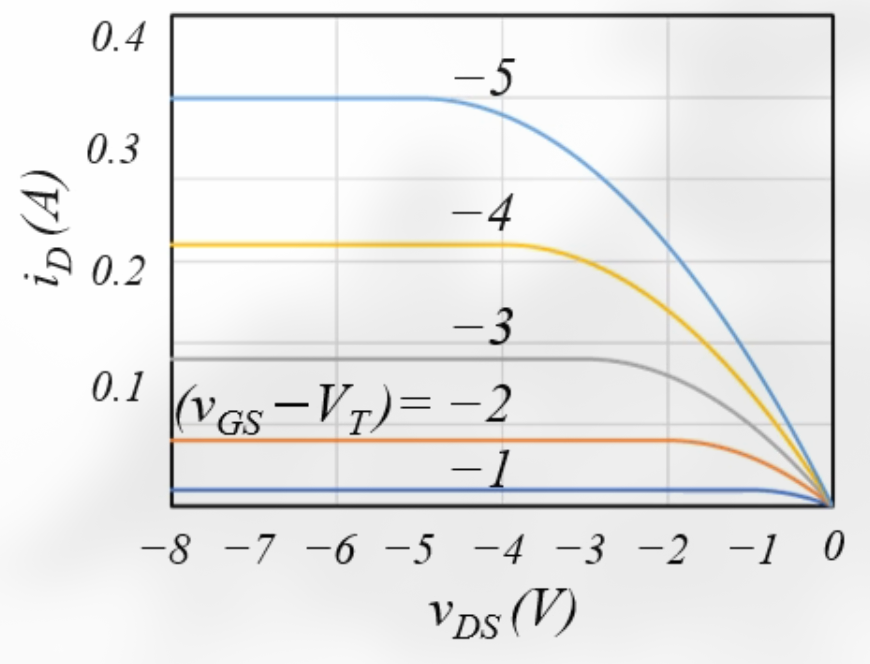
\includegraphics{output characteristics pmosfet.png}
\end{figure}
A negative bias on the gate will induce a channel of positive holes 
in the semiconductor, making the threshold voltage for a pMOSFET 
negative. Again, the normally on depletion mode pMOSFET graph has the same 
shape, but since there is an existing channel for current it will flow even for 
some positive values of $v_{GS}$. We need to deplete the channel by pushing away all 
the holes in it with the bias on the gate in order to turn it off. 

To review, there for four kinds of MOSFETs in which we are interested:
\begin{itemize}
    \item normally off, enhancement mode nMOSFETs
    \item normally on, depletion mode nMOSFETs
    \item normally off, enhancement mode pMOSFETs
    \item normally on, depletion mode pMOSFETs
\end{itemize}

\subsection{Transconductance}

Now, let us move on the the topic of transconductance. 
In the triode region, the transconductance is defined as 
\begin{equation} \label{eq:9}
    g_m = \frac{i_D}{v_{GS}} \rvert_{Q_{pt}}
\end{equation}
where 
\begin{equation}
    Q_{pt} = (I_D, V_{DS}).
\end{equation}
If we recall equation \ref{eq:5}, and substitute
for $i_D$ in equation \ref{eq:9}, then we obtain 
\begin{align}
    g_m &= \mu C_{ox} \frac{W}{L} v_{DS} \\
    &= \frac{i_{D(triode)}}{(v_{GS}-v_T)-\frac{v_{DS}}{2}}
\end{align}

In the saturation region, 
\begin{equation} \label{eq:10}
    g_m = \frac{di_D}{dv_{GS}} \rvert_{Q_{pt}}
\end{equation}
and 
\begin{equation} \label{eq:11}
    i_{D(sat)} = \mu C_{ox} \frac{W}{L} \frac{(v_{GS}-V_T)^2}{2}.
\end{equation}
Again combining these two equations, 
\begin{align} \label{eq:12}
    g_m &= \mu C_{ox} \frac{W}{L}(v_{GS} - V_T) \\
    &= \frac{2i_{D(sat)}}{(v_{GS}-V_T)}
\end{align}
The larger the transconductance, the larger 
the gain of an amplifier circuit 
that uses the transistor. 

\subsection{Channel length modulation}

By adjusting the voltage of the drain, we 
can modulate the channel length. Specifically, 
\begin{align} \label{eq:13}
    i_{D(sat)} &\propto \frac{1}{L-\Delta L} \\
    &\equiv \frac{1}{L}\left(1 + \frac{\Delta L}{L}\right).
\end{align}
And 
\begin{equation} \label{eq:14}
    \Delta L \propto (v_{DS} - v_{DS(sat)})
\end{equation}
means that 
\begin{equation} \label{eq:15}
    i_{D(sat)} = \frac{1}{2} \mu C_{ox} \frac{W}{L} (v_{GS}-V_T)^2 \left[1 + \lambda(v_{DS}-v_{DS(sat)})\right]
\end{equation}
where $\lambda$ is the empirically determined 
channel length modulation parameter. 
The output resistance at the drain is given by 
\begin{align} \label{eq:16}
    r_0 &= \left[\frac{\partial i_{D(sat)}}{\partial v_{DS}}\right]^{-1} \\
    &= \left[\lambda \frac{1}{2} k_n (v_{GS}-V_T)^2\right]^{-1} \\
    &= \frac{1}{\lambda I_{D(sat)}} \\
    &\approx \frac{V_A}{I_{D(sat)}}
\end{align}
Channel length modulation is not important when 
channel length is relatively large, but it is important 
on modern transistors where are on the order of nanometers. 

\subsection{MOSFETs in DC circuits}
Consider a circuit with two enhancement mode pMOSFETs. 
\begin{figure}
    \caption{MOSFET DC circuit}
    \label{fig:MOSFET DC circuit 1}
    \begin{center}
        \begin{circuitikz}
            \draw (0,0) node[nmos, left, xscale=-1] (m1) {};
            \node at (0,0) {$M_1$};
            \draw (m1.D) to ++(1,0);
            \draw[->] (m1.D) to ++(0,-0.25);
    
            \draw (2,0) node[nmos, left] (m2) {};
            \node at (2,0) {$M_2$};
            \draw[->] (m2.D) to ++(0,-0.25);
            \draw (m2.D) to ++(-1,0)
            to[short, -o] ++(0, 0.5) node[above] {$V^+$};
    
            \draw (m2.S) to[short, i=$I_{OUT}$] ++(0,-1);
            \draw (m2.G) to ++(0, -0.75)
            to (m1.S)
            to[R, i=$I_{REF}$, l=$R_{REF}$] ++(0,-1.5) node[ground] {};
        \end{circuitikz}
    \end{center}
\end{figure}
Notice that in figure \ref{fig:MOSFET DC circuit 1}, 
the drain of $M_1$ is directly attached to the gate. From 
this we have 
\begin{align} \label{eq:17}
    v_{DS1} &= v_{GS1} \\
    &= v_{GS2}
\end{align}
We are told $M_1$ is in saturation. If these are two identical 
transistors, then 
\begin{align} \label{eq:18}
    I_{REF} &= I_{D(sat)} \\
    &= \frac{1}{2} k_{p1} (v_{GS1} - V_{T1})^2\\
    &= I_{OUT}.
\end{align}
From this, we learn that the reference current 
is mirrored by the drain current if 
$k_{p1} = k_{p2}$ and $v_{GS1} = v_{GS2}$. 

Let us now look at the inverter shown in figure \ref{fig:MOSFET DC circuit 2}. 
\begin{figure}
    \caption{Inverter}
    \label{fig:MOSFET DC circuit 2}
    \begin{center}
        \begin{circuitikz}
            \draw (0,0) node[pmos, left] (m2) {};
            \node at (0,0) {$M_2$};
            \draw[->] (m1.D) to ++(0,-0.25);
            \draw (m2.D) to ++(0,-0.25);
            \node[left] at (m2.D) {$D_2$};
            \node[left] at (m2.S) {$S_2$};

            \draw[short, -o] (0,0.5) to ++(0, 1) node[above] {$5V$};
    
            \draw (0,-2) node[nmos, left] (m1) {};
            \node at (0,-2) {$M_1$};
            \node[left] at (m1.S) {$S_1$};
            \node[left] at (m1.D) {$D_1$};

            \draw (m1.D) to ++(0,0.25)
            to[short, -o] ++(0.5,0) node[right] {$V_{out}$};

            \draw[->] (m1.S) to ++(0,-0.125);
            \draw (0, -3) to[R] ++(0,-1) node[ground] {};

            \draw (m1.G) to ++(0,1);
            \draw (m2.G) to ++(0,-1)
            to[short, -o] ++(-1, 0) node[above] {$V_{in}$} node[below] {G};
        \end{circuitikz}
    \end{center}
\end{figure}
Let's try to find $V_{out}$ for $V_{in} = 0V$ and $V_{in} = 5V$. 
We are told that $V_{T(M1)} = 1V$ and $V_{T(M2)} = -1V$, because 
M1 is an enhancement mode nMOSFET and M2 is an enhancement mode 
pMOSFET. When $V_{in} = 0V$, M1 is off because $v_{GS1} < V_{T(M1)}$. 
Likewise, M2 is on because $v_{GS2} < V_{T(M2)}$ (recall that M2 is a pMOSFET).  
Since M1 is off, no current flows and $V_{out} = 5V$. For $V_{in} = 5V$, 
M1 flips on while M2 is off. Since M2 is off, no current flows. 
That means that $V_{out} = 5V$.

\subsection{Transistors as amplifiers}
The circuit shown in figure \ref{fig:Transistor as amplifier}
\begin{figure}
    \caption{Common-source nMOSFET amplifier circuit}
    \label{fig:Transistor as amplifier}
    \begin{center}
        \begin{circuitikz}
            \draw (0,0) node[nmos, left] (mos) {}
            (mos.G) to ++(-1,0)
            to[V, l=$v_{gs}$] ++(0,-1)
            to[V, l=$V_{GS}$] ++(0,-1)
            node[left] {$3.5 V$}
            to ++(2, 0)
            node[ground] {}
            to (mos.S);

            \node at (0, 3.2) {$V_{DD} = +10V$};
            \draw (0, 3) to[R, i=$i_D$, l=$R_D: 3.3k \Omega$, o-] (mos.D);
        \end{circuitikz}
    \end{center}
\end{figure}
has both AC and DC voltage sources. The source labelled 
by $V_{GS}$, all caps, is the DC voltage. The source 
$v_{gs}$, all lowercase, is the AC. This is not to be 
confused with $v_{GS}$, the total gate bias. The mix of 
cases indicates we have both AC and DC bias in consideration. 
The cool thing about this circuit is a small oscillation in 
the AC input induces a much larger oscillation in the 
output, hence calling it an amplifier. The output signal 
is going to be phase shifted by $180^\circ$. We can calculate the gain 
with eq. \ref{eq:19}
\begin{equation} \label{eq:19}
    A_v = \frac{v_{ds}}{v_{gs}}
\end{equation}
In this instance, 
\begin{align} \label{eq:20}
    A_v &= \frac{v_{ds}}{v_{gs}} \\
    &= \frac{4.17\angle 180^\circ}{1\angle 0^\circ} \\
    &= -4.17
\end{align}
This gain, however, will be somewhat distorted. To reduce distortion 
we need that $\lvert v_{gs} \rvert <<2(V_{GS}-V_T)$. The exact value 
of the "much less" symbol $<<$ will depend on the application, 
but it's common to require $\lvert v_{gs} \rvert < 0.2(V_{GS} - V_T)$. 
If we assume the small signal condition and no channel length modulation, then the transconductance
of the amplifier is 
\begin{equation} \label{eq:21}
    g_m = \sqrt{2k_n I_{D(sat)}}
\end{equation}

Figure \ref{fig:cs amplifier} shows the small signal equivalent circuit
of a common source amplifier. 
\begin{figure}
    \begin{center}
        \begin{circuitikz}
            \draw (4,-1) node[nmos] (mosfet) {};
            \draw (mosfet.S) -- ++(0,-0.1)
            -- ++(0, 0.6) 
            -- ++(-0.5,0)
            to[short, i=~] ++(0.5,0);

            \draw (0,0) to[V, invert, l=$V_{DD}$] ++(0,2)
            -- ++(4,0)
            to[R, i=$i_D$, l=$R_D$] (mosfet.D)
            ;
            \draw (mosfet.D) to[short, -o] ++(1,0) node[below] {$+$};
            \draw (mosfet.S) to ++(0,-1.25)
            to[short, -o] ++(1,0) node[above] {$-$}
            -- ++(-5, 0)
            -- ++(0,3);

            \node at (5, -1.5) {$v_{DS}$};

            \draw (mosfet.G) -- ++(-1,0)
            to[sV, l=$v_g$] ++(0, -1)
            to[V, l=$V_{GS}$] ++(0,-1)
            node[ground] {};
        \end{circuitikz}
    \end{center}
    \caption{Small signal equivalent circuit}
    \label{fig:cs amplifier}
\end{figure}
Notice the two voltage sources, one AC signal 
and one DC bias at the gate. The total 
input signal is given by
\begin{align} \label{eq:22}
    v_{GS}(t) &= v_{gs}(t) + V_{GS} \\
    v_{DS}(t) &= v_{ds}(t) + V_{DS}
\end{align}
The drain current for such a circuit 
when channel length modulation is accounted for 
is given by 
\begin{align*} \label{eq:23}
    i_{D(clm)} = \frac{1}{2}k_n \left[ v^2_{gs} + 2(V_{GS} - V_T)v_{gs} + (V_{GS} - V_T)^2 \right] \\
    \times \left[ 1 + \lambda(V_{DS} - (V_{GS} - V_T)) + \lambda(v_{ds} - v_{gs}) \right]
\end{align*}
When channel length modulation can 
be ignored, the current reduces to 
\begin{equation} \label{eq:24}
    i_{D(sat)} = \frac{1}{2}k_n \left[ v^2_{gs} + 2(V_{GS} - V_T)v_{gs} + (V_{GS} - V_T)^2 \right]
\end{equation}
For finite output resistance $r_0$, 
\begin{align} \label{eq:25}
    \frac{1}{r_0} &= \left[ \frac{\partial i_{D(clm)}}{\partial v_{DS}} \right] \\
    &= \frac{\partial}{\partial v_{DS}} \left\{ \frac{k_n}{2} (v_{GS} - V_T)^2 \left[ 1 + \lambda(v_{DS} - v_{DS(sat)}) \right] \right\} \\
    &= \frac{k_n}{2} (v_{GS} - V_T)^2 \frac{\partial}{\partial v_{DS}} \left[ 1 + \lambda(v_{DS} - v_{DS(sat)}) \right] \\
    &= \lambda \frac{k_n}{2} (v_{GS} - V_T)^2 \\
    &= \lambda I_{D(sat)}.
\end{align}
We then define the \emph{intrinsic voltage gain of a MOSFET}
as 
\begin{align} \label{eq:26}
    \mu_f &= g_m r_0 \\
    &= \sqrt{2k_n I_{D(sat)}} \left( \frac{1}{\lambda I_{D(sat)}} \right) \\
    &= \frac{1}{\lambda} \sqrt{\frac{2k_n}{I_{D(sat)}}}
\end{align}
We can greatly simplify circuit analysis 
by breaking the circuit up into 
AC and DC. To find the DC equivalent 
circuit, follow these steps: 
\begin{enumerate}
    \item Replace all capacitors with open circuits
    \item Replace all inductors with short circuits
    \item Deactivate AC sources 
    \item Find the Q-point using the DC equivalent circuit
\end{enumerate}
To find the AC equivalent circuit, 
\begin{enumerate}
    \item Replace all capacitors with short circuits at operational frequency
    \item Replace all inductors with open circuits at operational frequency
    \item Deactivate DC voltages and replace with short circuits 
    \item Deactivate DC current sources and replace with open circuits 
    \item Replace the transistor with its small-signal model 
\end{enumerate}

\subsection{Amplifier topologies}
There are three different nMOSFET amplifier 
topologies we will consider in this class, 
starting with the common-source amplifier shown in 
figure \ref{fig:common-source amplifier}. 
\begin{figure}
    \begin{center}
        \begin{circuitikz}
            \draw (0,0) node[nmos] (mosfet) {};
            \draw (mosfet.S) -- ++(0,-0.1)
            -- ++(0, 0.6) 
            -- ++(-0.5,0)
            to[short, i=~] ++(0.5,0);

            \node[ground] at (mosfet.S) {};

            \node[ground] at (-2, -1) {};
            \draw (-2, -1) to[V, l=$v_i$, invert] ++(0,1)
            to[short, -o, l=$v_g$] ++(1,0);
            
            \draw (mosfet.D) to[short, -o, l=$v_d$] ++(1,0)
            to[R, l=$R_L$, v=$v_0$] ++(0,-2)
            node[ground] {};
        \end{circuitikz}
    \end{center}
    \caption{Common-source amplifier}
    \label{fig:common-source amplifier}
\end{figure}
The common-source amplifier's input is taken 
through the gate, the output is taken 
through the drain, and the terminal that 
is common to output and input is the source. 

The second topology is the common-gate amplifier 
shown in figure \ref{fig:common-gate amplifier}.
\begin{figure}
    \begin{center}
        \begin{circuitikz}
            \draw (0,0) node[nmos] (mosfet) {};
            \draw (mosfet.S) -- ++(0,-0.1)
            -- ++(0, 0.6) 
            -- ++(-0.5,0)
            to[short, i=~] ++(0.5,0);

            \draw (mosfet.G) -- ++(-2, 0)
            node[ground] {};

            \node[ground] at (-2, -1.75) {};
            \draw (-2, -1.75) to[V, l=$v_i$, invert] ++(0,1)
            to[short, -o, l=$v_s$] ++(1,0)
            -- (mosfet.S);
            
            \draw (mosfet.D) to[short, -o, l=$v_d$] ++(1,0)
            to[R, l=$R_L$, v=$v_0$] ++(0,-2)
            node[ground] {};
        \end{circuitikz}
    \end{center}
    \caption{Common-gate amplifier}
    \label{fig:common-gate amplifier}
\end{figure}
Here we see that the AC voltage source is applied 
to the source, while the output is taken 
at the drain and the common terminal 
is at the gate. 

The previous two amplifiers suggest a 
third, the common-drain amplifier in 
figure \ref{fig:common-drain amplifier}.
\begin{figure}
    \begin{center}
        \begin{circuitikz}
            \draw (0,0) node[nmos] (mosfet) {};
            \draw (mosfet.S) -- ++(0,-0.1)
            -- ++(0, 0.6) 
            -- ++(-0.5,0)
            to[short, i=~] ++(0.5,0);

            \node[ground] at (-2, -1) {};
            \draw (-2, -1) to[V, l=$v_i$, invert] ++(0,1)
            to[short, -o, l=$v_g$] ++(1,0)
            -- (mosfet.G);
            
            \draw (mosfet.S) to[short, -o, l=$v_s$] ++(1,0)
            to[R, l=$R_L$, v=$v_0$] ++(0,-2)
            node[ground] {};

            \draw (mosfet.D) -- ++(1,0)
            node[ground] {};
        \end{circuitikz}
    \end{center}
    \caption{Common-drain amplifier}
    \label{fig:common-drain amplifier}
\end{figure}
As may be expected, here the common terminal 
is the drain, the input is at the gate, and 
the output is at the source. 

\marginnote{You may be thinking: "what happens if the 
input and output are swapped? Will the circuit still 
work as an amplifier?" No.} 

The voltage gain in a common-drain 
amplifier is given by 
\begin{equation} \label{eq:27}
    A_V = \frac{g_m R'_L}{1 + g_m R'_L} \left(\frac{R_G}{R_I + R_G}\right)
\end{equation}
where $R'_L = (r_0 || R_6 || R_3)$. 
For a MOSFET where $r_0 >> R_L$, 
\begin{equation} \label{eq:28}
    A_V \approx \frac{R_G}{R_I + R_G}
\end{equation}
When this is true, the MOSFET is 
acting as a \emph{voltage follower}. 

Figure \ref{fig:hybrid-pi model} shows the small-signal 
model for an nMOSFET called a hybrid-pi model. 
\begin{figure}
    \begin{center}
        \begin{circuitikz}
            \draw (0,0) node[left] {$G$}
            to[short, o-o] ++(1,0);
            
            \path (1.25,0) to[short, v=$v_{gs}$] ++(0,-2);

            \draw (1.25, -2) to[short, o-*] ++(2,0)
            to[short, -o] ++(0,-0.5)
            node[right] {$S$}
            -- ++(0,1)
            to[cI, l=$g_m v_{gs}$, invert] ++(0,1.5)
            -- ++(2,0)
            to[short, -o] ++(1,0)
            node[right] {$D$}
            to[short, i_=$i_d$] ++(-1,0)
            to[R, l=$r_0$] ++(0,-2)
            to[short, -o] ++(1,0)
            -- ++(-3,0);

            \path (6,0) to[short, v^=$v_ds$] ++(0,-2);
        \end{circuitikz}
    \end{center}
    \caption{Hybrid-pi model}
    \label{fig:hybrid-pi model}
\end{figure}
This model is excellent for 
common-source and common-drain amplifiers. 
For the common-gate amplifier, the alternative 
T-model shown in figure \ref{fig:T-model} is more useful. 
\begin{figure}
    \begin{center}
        \begin{circuitikz}
            \draw (0,0) node[left] {$G$}
            to[short, i=$i_g: 0$] ++(2,0)
            to[cI, invert, l=$g_m v_{gs}$] ++(0,2)
            to[short, -o] ++(0, 0.5)
            node[left] {D}
            to[short, i=$i_d$] ++(0,-0.5)
            -- ++(2,0)
            to[R, l=$r_0$] ++(0, -4)
            -- ++(-2,0)
            to[short, -o] ++(0,-0.5)
            node[right] {$S$}
            -- ++(0,0.5)
            to[R, l=$\frac{1}{g_m}$, v<=$v_{gs}$] ++(0,2);
        \end{circuitikz}
    \end{center}
    \caption{T-model}
    \label{fig:T-model}
\end{figure}
The voltage gain in a common-gate 
amplifier is given by 
\begin{equation} \label{eq:28}
    A_V = \frac{g_m R_L}{1 + g_m(R_I || R_6)} \left(\frac{R_6}{R_I+R_6}\right)
\end{equation}

Let's recap our three kinds of amplifiers.
For the inverting common-source amplifier, 
\begin{equation} \label{eq:29}
    A_V = -\frac{g_m R_L}{1 + g_m R_S} \left(\frac{R_G}{R_I+R_G}\right).
\end{equation}
Additionally, 
\begin{align} \label{eq:30}
    R_{in} &= \infty \\
    R_{out} &= R_L
\end{align}
For the non-inverting common-gate amplifier, 
\begin{equation} \label{eq:31}
    A_V = \frac{g_m R_L}{1 + g_m(R_I || R_6)} \left(\frac{R_6}{R_I+R_6}\right)
\end{equation}
with 
\begin{align} \label{eq:32}
    R_{in} &= \frac{1}{g_m} \\
    R_{out} &= R_L 
\end{align}
For the follower common-drain amplifier, 
\begin{align} \label{eq:33}
    A_V &= \frac{g_m R_L}{1 + g_m R_L} \left(\frac{R_G}{R_I+R_G}\right) \\
    &\approx \left(\frac{R_G}{R_I + R_G}\right). 
\end{align}
Here, 
\begin{align} \label{eq:34}
    R_{in} &= \infty \\
    R_{out} &= \frac{1}{g_m}
\end{align}

\subsection{Frequency range for FET amplifiers}

The \emph{lower-frequency cutoff} for an 
amplifier circuit is defined as the $\omega_L$ 
where the gain $A_V$ is $\frac{1}{\sqrt{2}}$
the maximum gain. 
We are told that 
\begin{align} \label{eq:omega_L}
    \omega_L &= \frac{1}{\tau} \\
    &= \frac{1}{r_{eq}C}.
\end{align}
If there are multiple capacitors in the circuit, 
find $r_{eq}$ for each, calculate all possible 
values of $\omega_L$, and pick the largest. 
The \emph{higher-frequency cutoff} $\omega_H$
is also defined as the frequency
where the gain $A_V$ is $\frac{1}{\sqrt{2}}$
the maximum gain, but the higher of the two 
values. 
For a common-source amplifier, 
\begin{equation} \label{eq:omega_H(cs)}
        \omega_H = \frac{1}{(R_S||R_1||R_2)C_{gs}}
\end{equation}
The bandwidth of useable frequencies is 
$\omega_H - \omega_L$. 

The higher-cutoff frequency is defined by capacitors within 
the amplifier circuit, $C_{gs}$ and $C_{gd}$. 
\marginnote{$C_{gs}$ is 
the capacitance between the gate and channel at a point 
nearer the source, while $C_{gd}$ is the same but 
for a point nearer the drain.}
We do not explore this relation within this course.
However, we are told the following equations are 
valid in the triode region:
\begin{align} \label{eq:35}
    C_{gc} &= WLC_{ox} \\
    C_{gd} &= \frac{C_{gc}}{2} + C_{gdo} X_{do} \\
    C_{gs} &= \frac{C_{gc}}{2} + C_{gso} X_{so}
\end{align}
\marginnote{$C_{gso}$ is the capacitance of oxide overlapping source, 
$C_{gdo}$ is the capacitance of oxide overlapping drain,
$X_{so}$ is the length of oxide overlap on source, 
and $X_{do}$ is the length of oxide overlap on drain.}
In the saturation region, 
\begin{align} \label{eq:36}
    C_{gd} &= C_{gdo}X_{do} \\
    C_{gs} &= \frac{2}{3}C_{gc} + C_{gso}X_{so}
\end{align}
Typically $C_{gd}$ is so much smaller than $C_{gs}$
as to be insignificant. 

The maximum useful linear frequency of 
a transistor is
\begin{align} \label{eq:37}
    f_T &= \frac{1}{2\pi} \frac{g_m}{C_{gc}} \\
    &= \frac{1}{2\pi} \frac{\mu}{L^2} (v_{gs} - V_T)
\end{align}

In addition to the intrinsic capacitances $C_{ox}$
and $C_d$, there are also parasitic capacitances. 
The junction capacitance $C_J$ forms between the 
source/drain and the semiconductor, while the 
overlap capacitance $C_{ov}$ forms between the 
source/drain and the metal contact on the gate. 

\newpage

\begin{figure}
    \begin{center}
        \begin{tabular}{ c | c }
            Region & Conditions \\
            \hline
            Cut-off & $v_{GS} < V_T$ \\
            Triode & $v_{DS} \leq v_{DS(sat)}$ \\
            Saturation & $v_{DS} > v_{DS(sat)}$ \\
            \hline
        \end{tabular}
    \end{center}
    \caption{nMOSFET regions of operation}
    \label{tab:nMOSFET regions}
\end{figure}

\begin{figure}
    \begin{center}
        \begin{tabular}{ c | c }
            Region & Conditions \\
            \hline
            Cut-off & $v_{GS} > V_T$ \\
            Triode & $v_{DS} \geq v_{DS(sat)}$ \\
            Saturation & $v_{DS} < v_{DS(sat)}$ \\
            \hline
        \end{tabular}
    \end{center}
    \caption{pMOSFET regions of operation}
    \label{tab:pMOSFET regions}
\end{figure}

\begin{figure}
    \begin{center}
        \begin{tabular}{ c | c | c }
            & nMOSFET & pMOSFET \\
            \hline
            Cutoff & $v_{GS} < 0$ & $v_{GS} > 0$ \\
            Triode & $v_{GS} > 0$ & $v_{GS} < 0$ \\
            Saturation & $v_{GS} > 0$ & $v_{GS} < 0$ \\
            \hline
            Enhancement & $V_T > 0$ & $V_T < 0$ \\
            Depletion & $V_T < 0$ & $V_T > 0$ \\
            \hline
        \end{tabular}
    \end{center}
    \caption{Differences between pMOSFET and nMOSFET}
    \label{tab:pn differences}
\end{figure}

\begin{figure}
    \begin{center}
        \begin{tabular}{ c | c | c }
             & nMOSFET & pMOSFET \\
            \hline 
            Enhancement &
            \begin{circuitikz}
                \draw (0,0) node[nmos] (mosfet) {};
                \draw (mosfet.D)node[right] {$V_{D}$};
                \draw (mosfet.S) node[right] {$V_S$}
                -- ++(0, 0.5) 
                -- ++(-0.5,0)
                to[short, i=~] ++(0.5,0);
                \draw (mosfet.G) node[left] {$V_{G}$};
            \end{circuitikz}
            & 
            \begin{circuitikz}
                \draw (0,0) node[pmos] (mosfet) {};
                \draw (mosfet.D) node[right] {$V_{D}$};
                \draw (mosfet.S) node[right] {$V_S$}
                -- ++(0, -0.5) 
                to[short, i=~] ++(-0.5,0);
                \draw (mosfet.G) node[left] {$V_{G}$};
            \end{circuitikz}
            \\
            \hline 
            Depletion & 
            \begin{circuitikz}
                \draw (0,0) node[nmosd] (mosfet) {};
                \draw (mosfet.D) node[right] {$V_{D}$};
                \draw (mosfet.S) node[right] {$V_S$}
                -- ++(0, 0.5) 
                -- ++(-0.5,0)
                to[short, i=~] ++(0.5,0);
                \draw (mosfet.G) node[left] {$V_{G}$};
            \end{circuitikz} 
            & 
            \begin{circuitikz}
                \draw (0,0) node[pmosd] (mosfet) {};
                \draw (mosfet.D) node[right] {$V_{D}$};
                \draw (mosfet.S) node[right] {$V_S$}
                -- ++(0, -0.5) 
                to[short, i=~] ++(-0.5,0);
                \draw (mosfet.G) node[left] {$V_{G}$};
            \end{circuitikz} 
            \\
        \end{tabular}
    \end{center}
    \caption{MOSFET schema}
    \label{tab:MOSFET schema}
\end{figure}

\begin{center}
    \begin{tabular}{ c | c  c }
        Equation & Condition & Reference \\
        \hline
        $v_{DS(sat)} = v_{GS} - V_T$ & MOSFET & \\
        \hline
        $i_{D(cutoff)} = 0$ & MOSFET & \\
        \hline
        $i_{D(triode)} = \mu C_{ox} \frac{W}{L} ((v_{GS}-V_T)v_{DS}-\frac{v^2_{DS}}{2})$ \\
        $= k_n ((v_{GS}-V_T)v_{DS}-\frac{v^2_{DS}}{2})$ \\
        $= \frac{k_n}{2} (2v_{DS(sat)} - v_{DS})v_{DS}$
        & MOSFET
        & eq. \ref{eq:5} \\
        \hline
        $i_{D(sat)} = \mu C_{ox} \frac{W}{L} \frac{(v_{GS}-V_T)^2}{2}$ \\
        $= k_n \frac{v^2_{DS(sat)}}{2}$
        & MOSFET
        & eq. \ref{eq:7} \\
        \hline
        $A_v = \frac{v_{out}}{v_{in}}$
        & Amplifying transistor
        & eq. \ref{eq:19} \\
        \hline
        $g_m = \sqrt{2k_n I_{D(sat)}}$ 
        & Amplifying transistor
        & eq. \ref{eq:21} \\
        \hline 
        $i_{D(clm)} = \frac{1}{2}k_n \left[ v^2_{gs} + 2(V_{GS} - V_T)v_{gs} + (V_{GS} - V_T)^2 \right]$ \\
        $\times \left[ 1 + \lambda(V_{DS} - (V_{GS} - V_T)) + \lambda(v_{ds} - v_{gs}) \right]$
        & CLM active 
        & eq. \ref{eq:24} \\
        \hline
        $\omega_L = \frac{1}{\tau}$ \\
        $= \frac{1}{r_{eq}C}$
        & Amplifier 
        & eq. \ref{eq:omega_L} \\
        \hline
        $\omega_H = \frac{1}{(R_S||R_1||R_2)C_{gs}}$
        & Common-source amplifier
        & eq. \ref{eq:omega_H(cs)} \\
        \hline
    \end{tabular}
\end{center}

\begin{figure}
    \begin{center}
        \begin{circuitikz}
            \draw (0,0) node[left] {$G$}
            to[short, o-o] ++(1,0);
            
            \path (1.25,0) to[short, v=$v_{gs}$] ++(0,-2);

            \draw (1.25, -2) to[short, o-*] ++(2,0)
            to[short, -o] ++(0,-0.5)
            node[right] {$S$}
            -- ++(0,1)
            to[cI, l=$g_m v_{gs}$, invert] ++(0,1.5)
            -- ++(2,0)
            to[short, -o] ++(1,0)
            node[right] {$D$}
            to[short, i_=$i_d$] ++(-1,0)
            to[R, l=$r_0$] ++(0,-2)
            to[short, -o] ++(1,0)
            -- ++(-3,0);

            \path (6,0) to[short, v^=$v_ds$] ++(0,-2);
        \end{circuitikz}
    \end{center}
    \caption{Hybrid-pi model}
\end{figure}
\begin{figure}
    \begin{center}
        \begin{circuitikz}
            \draw (0,0) node[left] {$G$}
            to[short, i=$i_g: 0$] ++(2,0)
            to[cI, invert, l=$g_m v_{gs}$] ++(0,2)
            to[short, -o] ++(0, 0.5)
            node[left] {D}
            to[short, i=$i_d$] ++(0,-0.5)
            -- ++(2,0)
            to[R, l=$r_0$] ++(0, -4)
            -- ++(-2,0)
            to[short, -o] ++(0,-0.5)
            node[right] {$S$}
            -- ++(0,0.5)
            to[R, l=$R_{in}: \frac{1}{g_m}$, v<=$v_{gs}$] ++(0,2);
        \end{circuitikz}
    \end{center}
    \caption{T-model}
\end{figure}

\pagebreak

\section{Operational Amplifier}
The \emph{operational amplifier} (op-amp)
is a high voltage gain amplifier
with a differential input. It can 
perform mathematical operations, 
but it's also commonly used in 
industrial and consumer products. 
On any op-amp pinout are eight terminals:
\begin{enumerate}
    \item offset null
    \item inverting input
    \item noninverting input
    \item negative power supply
    \item offset null
    \item output
    \item positive power supply 
    \item no connection
\end{enumerate}
The symbol for an op-amp 
is given in figure \ref{fig:op-amp symbol}.
\begin{figure}
    \begin{center}
        \begin{circuitikz}
            \draw (0, 0) node[op amp] (opamp) {};
            \node[left] at (opamp.+) {$v_+$};
            \node[left] at (opamp.-) {$v_-$};
            \node[right] at (opamp.out) {$V_{out}$};
            \draw[-latex] (opamp.up) -- +(0,1) node[above] (vv) {$V_+$};
            \draw[-latex] (opamp.down) -- +(0,-1) node[below] (v) {$V_-$};
        \end{circuitikz}
    \end{center}
    \caption{Operational amplifier symbol}
    \label{fig:op-amp symbol}
\end{figure}
We have a potential at the inverting terminal of
$v_-$, and a potential at the noninverting terminal of $v_+$. 
$V_-$ and $V_+$ are the negative and positive power supplies, 
respectively. 
We can model the op-amp as in figure \ref{fig:op-amp model}.
\begin{figure}
    \begin{center}
        \begin{circuitikz}
            \draw (0, 0) node[left] {$v_-$} 
            to[short, o-, i=$i_-$] ++(1,0)
            to[R, *-*, l=$R_i$, v<=$v_d$] ++(0,-2)
            to[short, -o, i<=$i_+$] ++(-1, 0)
            node[left] {$v_+$};

            \draw (5,0) to[R, o-, l=$R_0$] ++(-2,0)
            to[cV, l=$Av_d$] ++(0,-2)
            -- ++(1,0) node[ground] {}
            to[short, -o] ++(1,0);

            \path (4.5,0) to[short, v^=$v_0$] ++(0,-2);
        \end{circuitikz}
    \end{center}
    \caption{Operational amplifier model}
    \label{fig:op-amp model}
\end{figure}
The open-loop gain $A$ is typically $O(10^4)$, but 
can be higher or lower. The input signal 
is voltage, not current, so we typically 
make $R_i$ large to avoid loss of signal. 
\marginnote{In an ideal op-amp, $A = \infty$ and 
$R_i$ is also $\infty$.}
The maximum and minimum possible voltages 
are clipped to $V_+$ and $V_-$, respectively. 

Consider the feedback loop 
shown in figure \ref{fig:feedback loop}.
\tikzstyle{block} = [draw, fill=blue!20, rectangle, 
    minimum height=3em, minimum width=6em]
\tikzstyle{sum} = [draw, fill=blue!20, circle, node distance=1cm]
\tikzstyle{input} = [coordinate]
\tikzstyle{output} = [coordinate]
\begin{figure}
    \begin{center}
        \begin{tikzpicture}[auto, node distance=2cm,>=latex']
            \node [input, name=input] {};
            \node [sum, right of=input] (sum) {};
            \node [block, right of=sum, node distance=3cm] (system) {$A$};
            \node [output, right of=system] (output) {};
            \node [block, below of=system] (measurements) {$B$};
        
            \draw [draw,->] (input) -- node {$x_s$} (sum);
            \draw [->] (sum) -- node {$x_i$} (system);
            \draw [->] (system) -- node [name=y] {$x_o$}(output);
            \draw [->] (y) |- (measurements);
            \draw [->] (measurements) -| node[pos=0.99] {$-$} 
                node [near end] {$x_f$} (sum);
        \end{tikzpicture}
    \end{center}
    \caption{Feedback loop}
    \label{fig:feedback loop}
\end{figure}
Here, $x_o = Ax_i$ and $x_f = Bx_o$. At the 
summing circle, the feedback $x_f$ is subtracted 
from $x_s$ to yield $x_i$: $x_i = x_s - x_f$. 
We define the closed-loop gain as 
\begin{align} \label{eq:38}
    A_f &= \frac{x_o}{x_s} \\
    &= \frac{A}{1+AB}
\end{align}
The product $AB$ is the \emph{loop gain}, 
and $1 + AB$ is the \emph{amount of feedback}.
When $AB >> 1$, $A_f \approx \frac{1}{B}$. 
Consider the inverting op-amp shown in figure 
\ref{fig:inverting op-amp}.
\begin{figure}
    \begin{center}
        \begin{circuitikz}
            \draw (0, 0) node[op amp] (opamp) {};

            \draw (opamp.-) to[short] ++(-1,0) 
            node (a) {}
            to[R, l=$R_S$, i<=$I_S$] ++(-3,0)
            to[V, l=$V_S$] ++(0,-2)
            node[ground] {};

            \draw (a) -- ++(0,1)
            to[R, l=$R_f$] ++(3.4,0)
            to[short, i>=$I_f$] (opamp.out)
            to[short, -o] ++(0.5, 0)
            node[right] {$V_o$};

            \draw (opamp.+) -- ++(0,-1)
            node[ground] {};
        \end{circuitikz}
    \end{center}
    \caption{Inverting op-amp}
    \label{fig:inverting op-amp}
\end{figure}
Because the potential of the noninverting 
and inverting terminals of an op-amp
are equal, we know that $V_- = 0$. Ergo, 
\begin{equation} \label{eq:39}
    I_S = \frac{V_S}{R_S}
\end{equation}
With a little more algebra that makes a 
useful exercise for the reader, we obtain 
\begin{equation} \label{eq:40}
    A_f = -\frac{R_f}{R_S}
\end{equation}
Hence why this setup is called an inverting 
op-amp. 

\newpage

\subsection{Reference}

Ideal op-amp features:
\begin{itemize}
    \item $v_+ = v_-$
    \item $A = \infty$ 
    \item $R_o = 0$
    \item $i_- = i_+ = 0$
\end{itemize}

\pagebreak

\section{Circuit Analysis}

\subsection{Differential Equations}

An important function in circuit analysis 
is the exponential function 
\begin{equation} \label{eq:41}
    e^x = \sum_{k=0}^\infty \frac{x^k}{k!}
\end{equation}
Any function can be expressed as a linear 
combination of exponential functions. Recall 
also that $\int e^x dx = e^x + C$ and 
$\frac{d}{dx} e^x = e^x$. 
An \emph{ordinary differential equation} (ODE)
is given by 
\begin{equation} \label{eq:42}
    y(t) = \sum_{k=0}^{n} A_k \frac{d^k x(t)}{dt^k}
\end{equation}
$y(t)$ is the forcing function, our objective is 
to find $x(t)$ that matches $y(t)$. The process for 
this is to first solve the specific case 
when $y(t) = 0$, the homogeneous ODE. We then 
find the particular solution that matches $y(t)$. 
In the case of exponential circuit analysis, the homogeneous
case corresponds to analyzing our circuit absent 
any excitations from forcing functions. To make this clear,
we want to solve 
\begin{equation} \label{eq:43}
    0 = \sum_{k=0}^{n} A_k \frac{d^k x(t)}{dt^k}.
\end{equation}
We assume a solution of the form
\begin{equation} \label{eq:44}
    x_h(t) = Ae^{\lambda t}.
\end{equation}
Let's consider an example. Say 
\begin{equation}
    y(t) = 2x(t) + 3 \frac{dx(t)}{dt}.
\end{equation}
We take 
\begin{equation}
    0 = 2x_h(t) + 3 \frac{dx_h(t)}{dt}.
\end{equation}
If $x_h(t) = A e^{\lambda t}$, 
then 
\begin{equation}
    0 = 2A e^{\lambda t} + 3 A \lambda e^{\lambda t}.
\end{equation}
Cancelling out $Ae^{\lambda t}$ from 
both sides, we obtain 
\begin{equation}
    0 = 2 + 3 \lambda.
\end{equation}
This is the \emph{characteristic equation}
of the circuit. Solving this characteristic 
equation will provide the \emph{natural frequency}
$\lambda$ for the homogeneous ODE solution. 
\marginnote{$\lambda$ is called the 
natural frequency because it's what 
we get without any external excitation.}
Returning to our example, say 
$y(t) = 4e^{-t}$. We can reasonably 
assume that $x_p(t) = Be^{-t}$. 
Plugging this in, we find that 
\begin{align}
    y(t) &= 2x(t) + 3 \frac{dx(t)}{dt} \\
    4e^{-t} &= 2Be^{-t} + 3(-1)Be^{-t} \\
    B &= -4
    x_p(t) = -4e^{-t}.
\end{align}
The complete solution is the superposition 
of the homogeneous and particular solutions, 
\begin{equation}
    x(t) = x_h(t) + x_p(t).
\end{equation}
Recall that although we found $\lambda$ 
for the homogenous solution, we have not 
yet found $A$. To do so we require 
an initial condition. Say in this case 
the initial condition is given as 
$x(0) = 2$. Then 
\begin{align}
    x(0) &= 2 \\
    &= -4e^0 + Ae^0 \\
    A &= 6.
\end{align}
So the complete solution becomes 
\begin{equation}
    x(t) = -4r^{-t} + 6e^{-\frac{2}{3}t}
\end{equation}

\subsection{RC and RL Circuits}

This isn't a differential equations class, 
this is a circuits class. The reason 
we care about ODEs is because they arise 
in circuits. For example, consider 
the circuit in figure \ref{fig:RL circuit}.
\begin{figure}
    \begin{center}
        \begin{circuitikz}
            \draw (0,0) to[V, invert, l=$v_{in}$] ++(0,2)
            to[R, l=$R$] ++(2,0)
            to[L, l=$L$, v=$v_L(t)$, i=$i_L(t)$] ++(0,-2)
            -- ++(-2,0); 
        \end{circuitikz}
    \end{center}
    \caption{RL circuit}
    \label{fig:RL circuit}
\end{figure}
Remember that 
\begin{equation}
    v_L = L \frac{d i_L(t)}{dt}.
\end{equation}
Via KVL, we have that 
\begin{equation}
    v_{in}(t) = v_L(t) + Ri_L(t).
\end{equation}
Putting the two together, 
\begin{equation}
    v_{in}(t) = L \frac{d i_L(t)}{dt} + Ri_L(t).
\end{equation}
This is a first-order ODE. Solving it 
is left as an exercise to the reader. 
A similar process applies to the RC 
circuit shown in figure \ref{fig:RC circuit}.
\begin{figure}
    \begin{center}
        \begin{circuitikz}
            \draw (0,0) to[V, invert, l=$v_{in}$] ++(0,2)
            to[R, l=$R$] ++(2,0)
            to[C, l=$C$, v=$v_C(t)$, i=$i_C(t)$] ++(0,-2)
            -- ++(-2,0); 
        \end{circuitikz}
    \end{center}
    \caption{RC circuit}
    \label{fig:RC circuit}
\end{figure}
In both the RC and RL cases, solving the ODE 
will yield the formulas for $v_C(t)$ and 
$v_L(t)$ with which we are familiar from 
ECE 20001. 

Note that both the inductor and capacitor 
are non-ideal elements, and if we are to 
accurately model circuits we must account 
for this. Specifically, inductors behave 
non-ideally in the following ways:
\begin{itemize}
    \item The wire that makes up the coil 
    of the inductor has intrinsic resistance
    \item The spacing between the wire has 
    intrinsic capacitance 
    \item Hysteresis or eddy currents in the 
    ferrite core have intrinsic resistance
\end{itemize}
Capacitors have the following non-idea 
characteristics: 
\begin{itemize}
    \item The wire connected to the 
    capacitor has intrinsic inductance 
    \item The wire connected to the 
    capacitor has intrinsic resistance 
    \item  The insulating dielectric between 
    the plates of the capacitor has a large 
    but finite resistance, and leakage current 
    can therefore flow from one plate to another
\end{itemize}
The inductor is less ideal than the 
capacitor, since it necessarily has 
more non-ideal components than the 
capacitor. Therefore, for the capacitor, 
we can comfortably neglect the effects 
of the non-ideal wire. 
\marginnote{In real life, the effects of 
the wire can be minimized by using chip
capacitors, which have very short wires.}
Figures \ref{fig:non-ideal inductor}
and \ref{fig:non-ideal capacitor} show the 
non-ideal models for inductor and capacitor 
used in this course. 
\begin{figure}
    \begin{center}
        \begin{circuitikz}
            \draw (0,0) to[short, o-*, i=$i_L(t)$] ++(0,-1)
            -- ++(-1,0)
            to[L, l=$L$] ++(0,-1.5)
            to[R, l=$R_S$] ++(0,-1.5)
            -- ++(1,0)
            to[short, *-o] ++(0,-1)
            -- ++(0,1)
            -- ++(1,0)
            to[R, l=$R_P$, v<=$v_L(t)$] ++(0,3)
            -- ++(-1,0);
        \end{circuitikz}
    \end{center}
    \caption{Non-ideal inductor}
    \label{fig:non-ideal inductor}
\end{figure}
\begin{figure}
    \begin{center}
        \begin{circuitikz}
            \draw (0,0) to[short, o-*, i=$i_C(t)$] ++(0,-1)
            -- ++(-1,0)
            to[C, l=$C$] ++(0,-2)
            -- ++(1,0)
            to[short, *-o] ++(0,-1)
            -- ++(0,1)
            -- ++(1,0)
            to[R, l=$R_p$, v<=$v_C(t)$] ++(0,2)
            -- ++(-1,0);
        \end{circuitikz}
    \end{center}
    \caption{Non-ideal capacitor}
    \label{fig:non-ideal capacitor}
\end{figure}

\subsection{Switched Circuits}

The current through an inductor is continuous, 
even when the voltage across it is not. Likewise,
voltage across a capacitor is continuous even if 
current is not. Recall from ECE 20001 that the time 
it takes a variable of interest, inductor current 
or capacitor voltage, to go from $x(t_1)$ to $x(t_2)$
in its respective circuit is given by 
\begin{equation} \label{eq:45}
    t_2 - t_1 = \tau \ln{\left(\frac{x(t_1) - x(\infty)}{x(t_2) - x(\infty)}\right)}.
\end{equation}
If switched events are associated with $x(t)$, then 
eq. \ref{eq:45} can be used to find the time for which 
a certain circuit configuration is valid. 

Consider the circuit in figure \ref{fig:switched circuit}.
\begin{figure}
    \begin{center}
        \begin{circuitikz}
            \draw (0,0) to[V, invert, l=$12V$] ++(0,2)
            to[R, l=$6 k\Omega$] ++(2,0)
            to[nos] ++(0,-0.5)
            to[R, l_=$3 k\Omega$] ++(0,-1.5)
            -- ++(-2,0)
            -- ++(4,0)
            to[C, l=$0.5mF$, v<=$v_c(t)$] ++(0,2)
            -- ++(-2,0);
        \end{circuitikz}
    \end{center}
    \caption{Switched circuit}
    \label{fig:switched circuit}
\end{figure}
We are told that the switch is initially open 
as shown and closes when $v_c(t) = 9V$. The switch 
opens again when $v_c(t) = 5V$. $v_c(0^+) = 0V$. 
We wish to find an expression for $v_c(t)$ from $t=0$ 
to the third time the switch flips.  
Let's start by recalling the helpful equation in eq. \ref{eq:46}. 
\begin{equation} \label{eq:46}
    x(t) = x(\infty) + \left[x(t_0) - x(\infty)\right]e^{-\left(\frac{t-t_0}{\tau}\right)}
\end{equation}
Ergo, 
\begin{equation} \label{eq:47}
    v_c(t) = v_c(\infty) + \left[v_c(t_0) - v_c(\infty)\right]e^{-\left(\frac{t-t_0}{\tau}\right)}
\end{equation}
For an RC circuit such as this one, $\tau = RC$.
\begin{equation} \label{eq:48}
    v_c(t) = v_c(\infty) + \left[v_c(t_0) - v_c(\infty)\right]e^{-\left(\frac{t-t_0}{RC}\right)}
\end{equation}
We know from our conditions that $v_c(t_0) = 0$, so 
eq. \ref{eq:48} simplifies to
\begin{equation} \label{eq:49}
    v_c(t) = v_c(\infty) - v_c(\infty)e^{-\frac{t}{RC}}
\end{equation}
In the open configuration, $v_c(\infty) = 12V$ and $R = 6 k\Omega$.
We know that, but our circuit from $t = 0$ until $v_c(t) = 9V$ doesn't. 
Therefore, 
\begin{align}
    t_2 - t_1 &= \tau \ln{\left(\frac{x(t_1) - x(\infty)}{x(t_2) - x(\infty)}\right)} \\
    &= \tau \ln{\left(\frac{v_c(t_1) - v_c(\infty)}{v_c(t_2) - v_c(\infty)}\right)} \\
    t_2 &= RC \ln{\left(\frac{0 - 12}{9 - 12}\right)} \\
    &= 3 \ln{\left(\frac{-12}{-3}\right)} \\
    &\approx 4.16
\end{align}
and
\begin{align}
    v_c(t) &= v_c(\infty) - v_c(\infty)e^{-\frac{t}{RC}} \\
    &= 12 - 12e^{-\frac{t}{3}}
\end{align}
Now, let's consider what happens after the switch closes. 
Now $R = 6k\Omega || 3k\Omega = 2k\Omega$, and $v_c(t) = 4V$. 
This time around, $v_c(t_0) = 9V$. We therefore have 
\begin{align}
    t_2 - t_1 &= \tau \ln{\left(\frac{x(t_1) - x(\infty)}{x(t_2) - x(\infty)}\right)} \\
    t_2 - 4.16 &= \ln{\left(\frac{9-4}{5-4}\right)} \\
    t_2 &\approx 4.16 + 1.61 \\
    &= 5.77
\end{align}
and
\begin{align}
    v_c(t) &= v_c(\infty) + \left[v_c(t_0) - v_c(\infty)\right]e^{-\left(\frac{t-t_0}{\tau}\right)} \\
    &= 4 + \left[9 - 4\right]e^{-\left(\frac{t - 4.16}{1}\right)} \\
    &= 4 + 5e^{-(t - 4.16)}
\end{align}
Finally, the switch opens again. 
\begin{align}
    t_2 &= 5.77 + 3\ln{\left(\frac{5-12}{9-12}\right)} \\
    &= 8.31
\end{align}
and
\begin{equation}
    v_c(t) = 12 - 7e^{\left(-\frac{t-5.77}{3}\right)}
\end{equation}
Therefore, our complete function is 
\[v_c(t) = \begin{cases} 
      0 & t \leq 0 \\
      12 - 12e^{-\frac{t}{3}} & 0 \leq t \leq 4.16 \\
      4 + 5e^{-(t - 4.16)} & 4.16 \leq t \leq 5.77 \\
      12 - 7e^{\left(-\frac{t-5.77}{3}\right)} &  5.77 \leq t \leq 8.31
   \end{cases}
\]

\subsection{Second-order Differential Equations}

Consider the circuit shown in figure \ref{fig:LC circuit}.
\begin{figure}
    \begin{center}
        \begin{circuitikz}
            \draw (0,0) to[V, l=$v_{in}(t)$, invert] ++(0,2)
            to[L, l=$L$, i=$i(t)$] ++(3,0)
            to[C, l=$C$, v>=$v_C(t)$] ++(0,-2)
            -- ++(-3,0);
        \end{circuitikz}
    \end{center}
    \caption{LC circuit}
    \label{fig:LC circuit}
\end{figure}
By KVL, we see that 
\begin{equation}
    v_{in}(t) = v_C(t) + v_L(t)
\end{equation}
and we also know, 
because $i$ is the 
current through a capacitor, 
\begin{equation}
    i = C \frac{dv_C(t)}{dt}
\end{equation}
But wait! The voltage through 
the inductor is 
\begin{align}
    v_L(t) &= L \frac{di(t)}{dt} \\
    &= L \left(\frac{d}{dt} C \frac{dv_C(t)}{dt}\right)\\
    &= LC \frac{d^2 v_C(t)}{dt^2}.
\end{align}
That means 
\begin{equation}
    v_{in}(t) = LC \frac{d^2 v_C(t)}{dt^2} + v_C(t).
\end{equation}
Yikes. This is a second order 
homogeneous equation. We can 
still solve it by assuming 
a homogenous solution of the form 
\begin{equation}
    v_{ch} = Ae^{\lambda t},
\end{equation}
But now substitution and 
cancellation yields
\begin{equation}
    0 = LC \lambda^2 + 1
\end{equation}
as a characteristic equation, 
meaning
\begin{equation}
    \lambda = \pm j \frac{1}{\sqrt{LC}}.
\end{equation}
Well, this is no problem for us. 
To make things a little cleaner 
let's define $\omega_o = \frac{1}{\sqrt{LC}}$
as the \emph{natural frequency} of 
the LC circuit. Now what we have for 
a homogenous equation is 
\begin{equation}
    v_{ch} = A_1 e^{j\omega_ot} + A_2 e^{-j\omega_ot}
\end{equation}
Via Eurler's formula 
\begin{equation}
    e^{j\theta} = \cos{(\theta)} + j\sin{(\theta)},
\end{equation}
\marginnote{It's incredible how often 
Euler's formula arises 
in the natural world, isn't it?}
we have that 
\begin{equation}
    v_{ch}(t) = A_1 \left(\cos{(\omega_ot)} + j\sin{\omega_ot}\right)
    + A_2 \left(\cos{(-\omega_ot)} + j\sin{(-\omega_ot)}\right).
\end{equation}
With a little bit of 
algebraic manipulation, we find 
\begin{equation}
    v_{ch}(t) = B_1\cos{(\omega_ot)} + B_2 \sin{(\omega_ot)}.
\end{equation}
What that means for our circuit 
is that the capacitor's voltage will 
oscillate back and forth sinusoidally, 
which is a pretty cool result. 

\subsection{RLC circuits}

Let's now introduce a resistor 
to the LC circuit. Consider figure 
\ref{fig:RLC parallel circuit}, 
where resistor, inductor, and 
capacitor are in parallel. 
\begin{figure}
    \begin{center}
        \begin{circuitikz}
            \draw (0,0) -- ++(-2,0)
            to[R, l=$R$] ++(0,-2)
            -- ++(2,0)
            to[L, i<=$i_L(t)$, l^=$L$] ++(0,2)
            -- ++(2,0)
            to[C, l=$C$, v=$v_C(t)$] ++(0,-2)
            -- ++(-2,0);
        \end{circuitikz}
    \end{center}
    \caption{RLC parallel circuit}
    \label{fig:RLC parallel circuit}
\end{figure}
We can also align the components 
in parallel, like in figure \ref{fig:RLC series circuit}.
\begin{figure}
    \begin{center}
        \begin{circuitikz}
            \draw (0,0) to[R, l=$R$] ++(2,0)
            to[L, l=$L$] ++(2,0)
            to[short, i=$i_L(t)$] ++(0,-2)
            to[C, l=$C$, v>=$v_C(t)$] ++(-4,0)
            -- ++(0,2);
        \end{circuitikz}
    \end{center}
    \caption{RLC series circuit}
    \label{fig:RLC series circuit}
\end{figure}
In either case, the resistor dampens the sinusoidal 
response of the LC circuit. In the 
case of the parallel circuit of figure \ref{fig:RLC parallel circuit},
as the resistance goes to infinity, the circuit 
starts to resemble just a plain LC circuit. 
In the case of the series circuit of 
\ref{fig:RLC series circuit}, as the resistance 
goes to zero the circuit start to look more 
like an LC circuit. Deriving an ODE for 
both of these circuits is a wonderful 
exercise, give it a try and compare your result 
to the following expression.
\begin{equation}
    F = \frac{d^2 x(t)}{dt^2} + \frac{1}{\tau} \frac{dx(t)}{dt} + \frac{x(t)}{LC}
\end{equation}
where $\tau = \frac{L}{R}$ for series RLC circuits 
and $\tau = RC$ for parallel. 
\marginnote{Consider how $R$ affects 
the differential equation in both 
the series and parallel cases.}
Finding the solution to the differential is 
another great exercise. Here is the characteristic 
equation:
\begin{equation}
    0 = \lambda^2 + \frac{1}{\tau} \lambda + \frac{1}{LC}
\end{equation}
and here is the general solution
to the homogenous equation:
\begin{equation}
    x_h(t) = A_1 e^{\lambda_1 t} + A_2 e^{\lambda_2 t}
\end{equation}
Now the specific values of $\lambda$ 
become very relevant, and give us three cases. 
\begin{itemize}
    \item[\emph{Case 1: $\lambda$ real}]
    When $\lambda$s are real and distinct, the 
    circuit is \emph{overdamped}. There is 
    no oscillation, and the function simply goes to
    zero and stops. 
    \item[\emph{Case 2: both $\lambda$ identical}]
    When $\lambda_1 = \lambda_2$, the circuit 
    is \emph{critically damped}. The signal 
    in the circuit decays exponentially to zero. 
    \item[\emph{Case 3: $\lambda$ complex}] When $\lambda$ are complex, they will 
    be conjugates of one another and 
    the circuit is \emph{underdamped}. 
    If $\lambda$ is imaginary, then 
    the circuit has no dissipation and 
    will oscillate forever. If 
    $\lambda_1 = -\sigma_p \pm j\omega_d$ 
    and $\lambda_2 = -\sigma_p \mp j\omega_d$,
    then we say $\sigma_p$ is the attenuation 
    factor and $\omega_p$ is the dampened 
    resonance frequency. 
\end{itemize}
Figure \ref{fig:roots}
shows each case plotted on the complex plane. 
\begin{figure}
    \begin{center}
        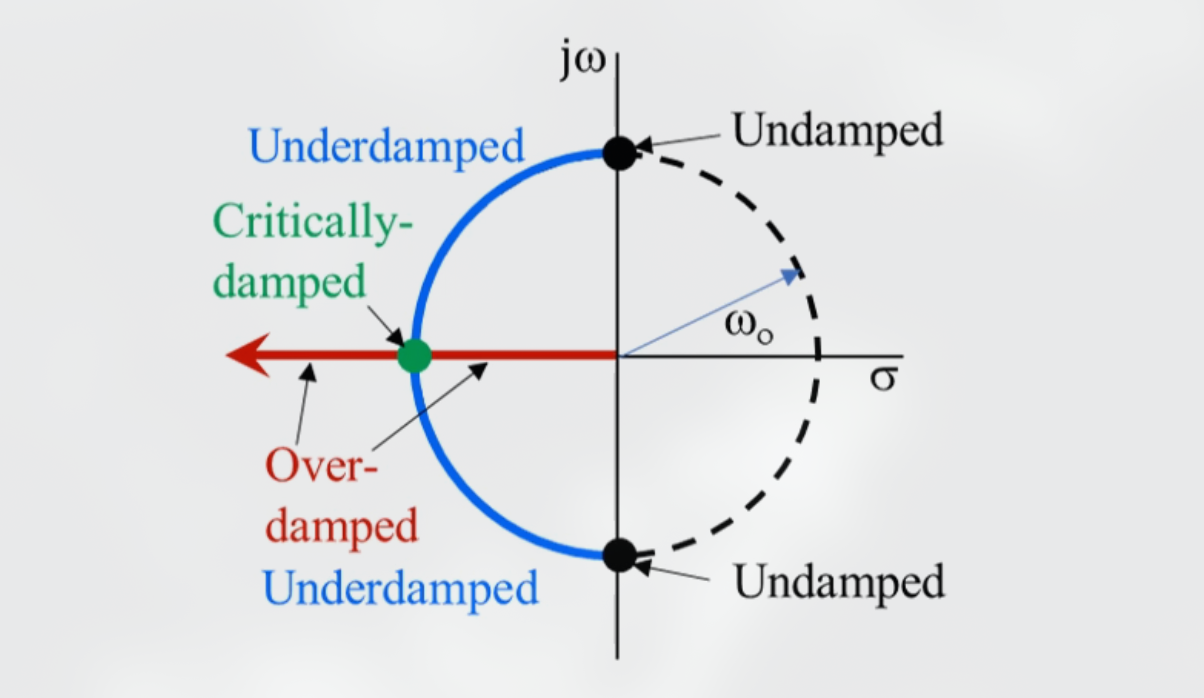
\includegraphics{images/roots.png}
    \end{center}
    \caption{Damping cases on complex plane}
    \label{fig:roots}
\end{figure}

\subsection{Convolution}

Given two functions, $f(t)$ and $g(t)$, their 
\emph{convolution} is 
\[f(t) * g(t) = \int_{-\infty}^{\infty} f(\tau)g(t-\tau)d\tau.\]
A notable property of the Dirac delta function 
$\delta(t)$ is that 
\begin{align} \label{eq:convolution with delta}
    f(t) * \delta(t) &= \int_{-\infty}^{\infty} f(\tau)\delta(t-\tau)d\tau \\
    &= f(t)
\end{align}
Additionally, 
\begin{align} \label{eq:time-shift convolution}
    f(t) * \delta(t - T) &= \int_{-\infty}^{\infty} f(\tau)\delta(t-T-\tau)d\tau \\
    &= f(t - T)
\end{align}
It may seem a bit odd to convolve a function 
when you can just compute it, but soon we shall 
find examples where convolution is actually 
easier than finding the function $f(t)$, and then 
we will be glad for eqs. \ref{eq:convolution with delta}
and \ref{eq:time-shift convolution}.
If we convolve $f(t)u(t)$ with $u(t)$, we obtain 
\begin{align}
    f(t)u(t) * u(t) &= \int_{-\infty}^{\infty} f(\tau)\delta(\tau)u(t-\tau)d\tau \\
    &= \int_{0}^{t} f(\tau) d\tau
\end{align}
which is simply the integral of $f(t)$. 
Convolution is, as can be shown with a bit of elbow 
grease, commutative, associative, and distributive 
over addition. 

\subsection{Linear Time Invariant Systems}

Again, however, this is an electrical engineering class, 
not a math class. How does this relate to circuits?
For the purposes, of this class, it allows us 
to relate outputs to inputs using 
functions that describe a linear network. 
Specifically, we can model 
\emph{linear time invariant} (LTI) systems, 
which produce output signals
that are related to inputs in a 
linear and time invariant manner.
Recall that linear means the differential 
equation has the form 
\[b(x) = a_0(x)y + a_1(x)\frac{dy}{dx} + a_2\frac{d^2 y}{dx^2} + \dots + a_n(x)\frac{d^n y}{dx}.\]
The \emph{degree} of this differential
equation is $n$, but it's linear because 
$b(x)$ is a linear combination 
of derivatives of $y$. Likewise, 
\[\frac{1}{L} \frac{dv_{in}(t)}{dt} = \frac{d^2 i_L(t)}{dt^2} + \frac{R}{L} \frac{di_L(t)}{dt} + \frac{1}{LC}i_L(t)\]
is linear, even though its \emph{order} is two. 
That's the linear part of linear 
time invariant. The time invariant 
part means that whether we apply an 
input to the system now or 
$T$ seconds from now, the output 
will be identical except for a 
time delay of $T$ seconds. 
That is, if the output due to 
input $x(t)$ is $y(t)$, then the 
output due to input $x(t - T)$ is $y(t - T)$. 
Hence, the system is time invariant 
because the output does not depend on 
the particular time the input is applied.

Suppose we have some LTI system, 
where the input is $x(t)$ and the 
output is $y(t)$. The relationship 
betwen them is given by $x(t) * h(t) = y(t)$. 
$h(t)$ is the \emph{impulse response}. 
Consider the case of the RC circuit in figure \ref{fig:RC LTI}. 
\begin{figure}
    \begin{center}
        \begin{circuitikz}
            \draw (0,0) to[V, invert, l=$v_{in}(t)$] ++(0,2)
            to[R, l=$R$, i=$i_C(t)$] ++(2,0)
            to[C, v^=$v_{out}(t)$] ++(0,-2)
            -- ++(-2,0);
        \end{circuitikz}
    \end{center}
    \caption{RC circuit as an LTI system}
    \label{fig:RC LTI}
\end{figure}
For convenience, let $R = 1\omega$ and 
$C = 1F$. Let the circuit also be at 
rest at $t_0 = 0$. We know that for an RC circuit, 
\[v_c(t) = v_c(\infty) + [v_c(t_0) - v_c(\infty)] e^{-\frac{t-t_0}{RC}}\]
In this case, $v_C(t) = v_{out}(t)$, 
$v_{out}(t_0) = 0V$, and by inspection 
$v_C(\infty) = v_{in}(t)$. Our equation becomes 
\[v_{out}(t) = v_{in}(t) - v_{in}(t)e^{-t}.\]
Let's let $v_{in}(t) = u(t)$. Then 
\[u(t) = (1-e^{-t})u(t).\]
If we differentiate both sides, 
then we have that 
\begin{align}
    \frac{d}{dt} u(t) &= \frac{d}{dt} u(t) - \frac{d}{dt} e^{-t}u(t) \\
    \delta(t) &= \delta(t) - (e^{-t}\delta(t) - e^{-t}u(t)) \\
    &= e^{-t}u(t) \\
    &= h(t)
\end{align}
The response of the circuit to a Dirac impulse excitation is
found by taking the time derivative of the unit-step response.
That's important: the impulse response is 
the derivative of the step response. 

\subsection{Laplace Transformations}

I don't know about you, but my idea of a 
good time isn't sitting down to solve 
integro-differential equations. Luckily
there's a better way to solve circuits. 
If we can move 
from the time domain to the frequency 
domain our math gets a lot easier 
and we'll have time for more important things,
such as literally anything else. 
Enter the one-sided \emph{Laplace transform}. 
This is big kid math and you should be excited
because it turns nasty differential equations 
into nice algebraic ones. Eq. \ref{eq:laplace} 
shows the guts of the Laplace transform. 
\begin{align} \label{eq:laplace}
    \mathcal{L}\left\{f(t)\right\} &= F(s) \\
    &= \int_{0}^{\infty} f(t)e^{-st}dt
\end{align}
The Laplace transform turns a function 
of time $t$ into a function of 
frequency $s$ by integrating time away. 
Eq. \ref{eq:laplace derivative} shows why that's useful. 
\begin{align} \label{eq:laplace derivative}
    \mathcal{L}\left\{\frac{d}{dt} f(t)\right\} &= \int_{0}^{\infty} \frac{d}{dt} f(t)e^{-st}dt \\
    &= e^{-st}f(t) \rvert_{t=0}^{\infty} - \int_{0}^{\infty} -s f(t)e^{-st}dt \\
    &= s \mathcal{L}\left\{f(t)\right\} - f(0)
\end{align}
Did you catch that? We transformed a 
differential equation into an algebraic one. 
With the help of a table like table \ref{tab:laplace}, we can transform 
back into the time domain too. 
\marginnote{Technically, you don't need a table.
The inverse Laplace transform is defined as 
$\mathcal{L}^{-1} \{F(s)\}(t) =  \frac{1}{2\pi i}\lim_{T\to\infty}\int_{\gamma-iT}^{\gamma+iT}e^{st}F(s)\,ds$,
but like, gross.}

Let's see this applied to a circuit. Say we have 
an RC circuit with $v_{in} = Au(t)$, where 
$A$ is constant. We know that 
\[RC \frac{d}{dt}v_C(t) + v_C(t) = Au(t).\]
While we could solve this with our ordinary 
differential methods, we're better than that now. 
Take the Laplace transform of both sides. 
\begin{align}
    \mathcal{L}\left\{RC \frac{d}{dt}v_C(t) + v_C(t)\right\} &= \mathcal{L}\left\{Au(t)\right\} \\
    \mathcal{L}\left\{RC \frac{d}{dt}v_C(t)\right\} + \mathcal{L}\left\{v_C(t)\right\} &= \mathcal{L}\left\{Au(t)\right\} \\
    RC \left(sV_C(s)-v_C(0)\right) + V_C(t)&= \frac{A}{s} \\
    V_C(s) &= \frac{A}{RC}\left(\frac{1}{s(s+\frac{1}{RC})}\right) + \frac{v_C(0)}{s + \frac{1}{RC}} \\
    &= \frac{A}{s} - \frac{A}{s+\frac{1}{RC}} + \frac{v_C(0)}{s+\frac{1}{RC}} \\
    \mathcal{L}\left\{V_C(s)\right\} &= \mathcal{L}\left\{\frac{A}{s} - \frac{A}{s+\frac{1}{RC}} + \frac{v_C(0)}{s+\frac{1}{RC}}\right\} \\
    &= \mathcal{L}\left\{\frac{A}{s}\right\} - \mathcal{L}\left\{\frac{A}{s+\frac{1}{RC}}\right\} + \mathcal{L}\left\{\frac{v_C(0)}{s+\frac{1}{RC}}\right\} \\
    &= A(1-e^{-\frac{t}{RC}})u(t) + v_C(0)e^{-\frac{t}{RC}}u(t)
\end{align}
Isn't that so much \emph{easier}? 
In all seriousness, computers are 
much better at algebra than calculus, 
so it's methods like the Laplace
transform that allow computational
tools for solving circuits to exist. 

Let's tie convolutions and Laplace 
transforms together now. Say we take the 
Laplace transform of two functions 
$f(t)$ and $g(t)$, both of which 
are $0$ for $t < 0$. We can write them 
as $f(t)u(t)$ and $g(t)u(t)$, and we 
will. Now, the Laplace transform 
of their convolution is 
\begin{align}
    \mathcal{L} \left\{f(t)*g(t)\right\} &= \int_0^{\infty} \int_{-\infty}^{\infty} f(\tau)g(t-\tau)d\tau e^{-st}dt \\
    &= \int_0^{\infty} \int_{-\infty}^{\infty} f(\tau)u(t) g(t-\tau)d\tau e^{-st}dt \\
    &= \int_0^{\infty} \int_{0}^{\infty} f(\tau) g(t-\tau)d\tau e^{-st}dt \\
    &= \int_0^{\infty} f(\tau) \int_{0}^{\infty} g(t-\tau) e^{-st}dt d\tau \\
    \lambda &= t - \tau \\
    \mathcal{L} \left\{f(t)*g(t)\right\} &= \int_0^{\infty} f(\tau) \int_{0}^{\infty} g(\lambda) e^{-s(\lambda+\tau)}d\lambda d\tau \\
    &= \int_0^{\infty} f(\tau) \int_{0}^{\infty} g(\lambda) e^{-s\lambda}e^{-s\tau}d\lambda d\tau \\
    &= \int_0^{\infty} f(\tau)e^{-s\tau}d\tau \int_{0}^{\infty} g(\lambda) e^{-s\lambda}d\lambda \\
    &= F(s)G(s)
\end{align}
So convolution in the time domain corresponds 
to multiplication in the frequency domain.

Since computing the inverse Laplace 
is so unattractive, we generally 
seek a way to break our function
into pieces so we can use a table 
lookup on each piece. 
A Laplace transform, can always be represented as 
\[F(s) = \frac{a_0 + a_1s + a_2s^2 + \dots + a_m s^m}{b_0 + b_1s + b_2s^2 + \dots + b_n s^n},\]
where $a_i, b_i$ are real and rational
and $m \leq n$. Think about it, have 
you ever seen a Laplace transform 
where the numerator was a higher
degree than the denominator? 
The reason we care about that is because it
enables us to write our transform as 
\[F(s) = A_0 + \frac{A_1}{s-p_1}+\frac{A_2}{s-p_2}+\dots+\frac{A_m}{s-p_n}\]
using partial fraction expansion. Via 
the linearity of the Laplace transform, 
we can then change each individual addend 
back into its respective time-domain counterpart. 
We have three cases to consider. 
\begin{enumerate}
    \item[Case 1:] The denominator 
    has real, distinct roots. In 
    this case the transform can be
    expressed as 
    \begin{align} \label{eq:distinct real roots}
        F(s) &= \frac{a_0+a_1s+a_2s^2+\dots+a_ms^m}{(s-p_1)(s-p_2)\dots (s-p_n)} \\
        &= A_0 + \sum_{k=1}^{n} \frac{A_k}{s-p_k}.
    \end{align}
    To find any $A_i$, simply multiply both sides 
    of eq. \ref{eq:distinct real roots} by $(s-p_i)$.
    You'll obtain 
    \begin{equation}
        \frac{a_0+a_1s+a_2s^2+\dots+a_ms^m}{(s-p_1)\dots (s-p_{i-1}) (s-p_{i+1}) \dots (s-p_n)} = (s-p_i) \left(A_0 + \sum_{k \neq i}^{n} \frac{A_k}{s-p_k}\right) + A_i
    \end{equation}
    Then set $s$ equal to $p_i$ to obtain
    \begin{equation}
        \frac{a_0+a_1p_i+a_2p^2_i+\dots+a_mp^m_i}{(p_i-p_1)\dots (p_i-p_{i-1}) (p_i-p_{i+1}) \dots (p_i-p_n)} = A_i.
    \end{equation}
    Repeat for all $p_i$ to find all $A_i$. 
    \item[Case 2:] The denominator has 
    real, repeated roots. This would look 
    something like 
    \begin{align} \label{repeated real roots}
        F(s) &= \frac{a_0+a_1s+a_2s^2+\dots+a_ms^m}{(s-p_1)(s-p_1)\dots (s-p_n)} \\
        &= \frac{A_1}{s-p_1} + \frac{A_2}{(s-p_1)^2} + \sum_{k=3}^{n} \frac{A_k}{s-p_k}.
    \end{align}
    The same process as in case 
    1 will take care of this. 
    To find $A_2$, multiply 
    both sides of eq. \ref{repeated real roots} 
    by $(s-p_1)^2$ and set $s = p_1$. Proceed as 
    before. 
    \item[Case 3:] The denominator 
    has complex roots. If you're unlucky, 
    you'll have to write your Laplace 
    transform as 
    \begin{align} \label{eq:complex roots}
        F(s) &= \frac{a_0+a_1s+a_2s^2+\dots+a_ms^m}{((s+\sigma)^2 +\omega^2) \dots (s-p_n)} \\
        &= \frac{a_0+a_1s+a_2s^2+\dots+a_ms^m}{(s + \sigma + j\omega)(s + \sigma -j\omega)\dots (s-p_n)} \\
        &= \frac{A_1 + jA_2}{s+\sigma+j\omega} + \frac{A_1-jA_2}{s+\sigma-j\omega} + \text{real roots}.
    \end{align}
    In this case, find the real roots 
    with whichever of the two previous 
    cases is applicable and then multiply 
    by $s+\sigma+j\omega$ and $s+\sigma+j\omega$ 
    to solve for the imaginary roots. 
\end{enumerate}

\pagebreak

\subsection{Reference}

\newcounter{NumberInTable}
\newcommand{\LTNUM}{\stepcounter{NumberInTable}{(\theNumberInTable)}}
\newcommand{\Laplace}[1]{\ensuremath{\mathcal{L}{\left[#1\right]}}}
\newcommand{\InvLap}[1]{\ensuremath{\mathcal{L}^{-1}{\left[#1\right]}}}
\vspace{2ex}
\begin{center}
    \begin{table}
        \caption{Laplace transforms}
        \label{tab:laplace}
        \begin{tabbing}
            \hspace*{1.5 in}\=\hspace{1.5in}\= \kill
            $f(t)$ \> $\Laplace{f(t)}=F(s)$ \> \\ \\
            $1$       			 \> $\dfrac{1}{s}$           \>\LTNUM \\ \\
            $e^{at}f(t)$	\> $F(s-a)$	\>\LTNUM \\ \\ 
            $u(t-a)$ \> $\dfrac{e^{-as}}{s}$ \>\LTNUM \\ \\
            $f(t-a)$ \> $e^{-sa}F(s)$ \>\LTNUM \\ \\
            $\delta(t-t_0)$ \> $e^{-st_0}$ \>\LTNUM \\ \\
            $t^nf(t)$ 	\> $(-1)^n\dfrac{d^nF(s)}{ds^n}$  \>\LTNUM \\ \\
            $f'(t)$ 	\> $sF(s) - f(0)$ \>\LTNUM \\ \\
            $f^{n}(t)$ 	\> $s^nF(s) - s^{(n-1)} f(0) - $ \\ \\
            \> $\cdots - f^{(n-1)}(0)$ \>\LTNUM \\ \\
            $f(t)*g(t)$ \> $F(s)G(s)$ \>\LTNUM \\ \\
            $t^n$ ($n=0,1,2,\dots$)     \> $\dfrac{n!}{s^{n+1}}$    \>\LTNUM \\ \\
            $\sin kt$ 	\> $\dfrac{k}{s^2+k^2}$ \>\LTNUM \\ \\
            $\cos kt$ 	\> $\dfrac{s}{s^2+k^2}$ \>\LTNUM \\ \\
        \end{tabbing}
    \end{table}
\end{center}

\pagebreak

\section{Advanced circuit analysis}

\subsection{Impedance, Admittance, and Zero-State Response}
We're engineers. We're all about 
making things easier, so even 
though Laplace transforms have 
greatly simplified our differential 
equations, we'd still like to 
find an easier method to 
analyze linear circuits. That 
is precisely what impedance will 
allow us to do. 

Let's think about the current-voltage 
relationships for our three major 
components. 
\begin{itemize}
    \item[Resistors:] 
    \begin{equation}
        \mathcal{L}\left\{v_R(t) = Ri_R(t)\right\} = RI_R(s)
    \end{equation}
    \begin{equation}
        \mathcal{L}\left\{i_R(t) = Gv_R(t)\right\} = GV_R(s)
    \end{equation}
    \item[Inductors:] 
    \begin{align}
        \mathcal{L}\left\{v_L(t) = L\frac{di_L(t)}{dt}\right\} &= V_L(s) \\
        &= L\left(sI_L(s) - i_L(0)\right)
    \end{align}
    \begin{align}
        \mathcal{L}\left\{i_L(t) = \frac{1}{L} \int_{-\infty}^{t}v_L(\tau) d\tau\right\} &= I_L(s) \\
        &= \frac{1}{L} \left(\frac{V_L(s)}{s} + \frac{\int_{-\infty}^{0} v_L(\tau) d\tau}{s}\right)
    \end{align}
    \item[Capacitors:]
    \begin{align}
        \mathcal{L}\left\{v_c(t) = \frac{1}{C} \int_{-\infty}^{t}i_C(\tau) d\tau\right\} &= V_C(s) \\
        &= \frac{1}{C} \left( \frac{I_C(s)}{s} + \frac{\int_{-\infty}^{0} i_C(\tau) d\tau}{s}\right)
    \end{align}
    \begin{align}
        \mathcal{L}\left\{i_c(t) = C \frac{dv_c(t)}{dt}\right\} &= I_C(s) \\
        &= C\left(sV_C(s) - v_C(0)\right)
    \end{align}
\end{itemize}

The \emph{zero-state response} is the response of the circuit 
to external sources when its initial conditions are zero. 
If we have zero-state conditions, then 
\begin{itemize}
    \item[Resistors:] $V_R(s) = RI_R(s)$
    \item[Inductors:] $V_L(s) = sLI_L(s)$
    \item[Capacitors:] $V_C(S) = \frac{I_C(s)}{sC}$
\end{itemize}
We can generalize the concept of resistance 
to the complex world by defining the impedance $Z$ as
\[Z(s) = \frac{V(s)}{I(s)}.\]
That makes the impedance for each element 
\begin{itemize}
    \item[Resistors:] $Z_R(s) = R$
    \item[Inductors:] $Z_L(s) = sL$
    \item[Capacitors:] $Z_C(s) = \frac{1}{sC}$   
\end{itemize}
Under zero-state conditions, the current 
for each element is given by 
\begin{itemize}
    \item[Resistors:] $I_R(s) = \frac{V_R(s)}{R}$
    \item[Inductors:] $I_L(s) = \frac{V_L(s)}{sL}$
    \item[Capacitors:] $I_C(s) = sCV_C(s)$  
\end{itemize}
The admittances for each passive element are 
\begin{itemize}
    \item[Resistors:] $Y_R(s) = \frac{1}{R}$
    \item[Inductors:] $Y_L(s) = \frac{1}{sL}$
    \item[Capacitors:] $Y_C(s) = sC$  
\end{itemize}
The concepts of impedance and admittance 
are extremely attractive because they allow 
us to sidestep the use of differential 
equations and solve our circuits linearly. 
We can basically treat impedance in the frequency 
realm as we would resistance in the time realm. 
Here, let's have an example. 
\begin{figure}
    \begin{center}
        \begin{circuitikz}
            \draw (0,0) to[V, invert, l=$5u(t)V$] ++(0,2)
            to[R, l=$100\Omega$] ++(2,0)
            to[C, l_=$0.1F$, v^=$v_C(t)$] ++(0,-2)
            -- ++(-2,0);
        \end{circuitikz}
    \end{center}
    \caption{Time domain}
    \label{fig:time domain}
\end{figure}
In the frequency domain, figure \ref{fig:time domain}
becomes \ref{fig:freq domain}.
\begin{figure}
    \begin{center}
        \begin{circuitikz}
            \draw (0,0) to[V, invert, l=$\frac{5}{s}$] ++(0,2)
            to[R, l=$100\Omega$] ++(2,0)
            to[C, l_=$\frac{10}{s}$, v^=$V_C(t)$] ++(0,-2)
            -- ++(-2,0);
        \end{circuitikz}
    \end{center}
    \caption{Frequency domain}
    \label{fig:freq domain}
\end{figure}
Since we can treat impedance like resistance, let's 
do a simple voltage division to solve for $V_C(s)$ 
(and subsequently, $v_C(t)$).
\begin{align}
    V_C(s) &= \frac{Z_C}{Z_C + Z_R} V_{in}(s) \\
    &= \frac{\frac{10}{s}}{\frac{10}{s} + 100} \frac{5}{s} \\
    &= \frac{5}{s(10s+1)} \\
    &= \frac{0.5}{s(s+\frac{1}{10})} \\
    &= \frac{A}{s} + \frac{B}{s + \frac{1}{10}} \\
    &= \frac{5}{s} - \frac{5}{s+\frac{1}{10}}.
\end{align}
If we take the inverse Laplace transform of both 
sides, we find that 
\begin{align}
    \mathcal{L}^{-1}\left\{ V_C(s) \right\} &= \mathcal{L}^{-1}\left\{ \frac{5}{s} \right\} - \mathcal{L}^{-1}\left\{ \frac{5}{s+\frac{1}{10}} \right\} \\
    &= v_C(t) \\
    &= 5u(t) - 5e^{-\frac{t}{10}}u(t) \\
    &= (5 - 5e^{-\frac{t}{10}})u(t)
\end{align}
Exactly the result we would achieve 
using differential equations or Laplace 
transforms, with arguably much less 
work. However, we assumed zero-state 
conditions. Can this method deal 
with situations where the initial 
state is not zero? Yes! 
Consider again figure \ref{fig:freq domain}, 
but this time say $v_C(0) = 2V$. 
We'll use KVL around the circuit to obtain 
\begin{align}
    V_{in}(s) &= V_R(s) + V_C(s) \\
    &= RI_C(s) + V_C(s) \\
    &= RC\left(sV_C(s) - v_C(0)\right) + V_C(s) \\
    \frac{5}{s} &= 10\left(sV_C(s) - 2\right) + V_C(s).
\end{align}
If we solve for $V_C(s)$, we find 
that 
\begin{equation}
    V_C(s) = \frac{5}{s} - \frac{3}{s+0.1},
\end{equation}
making our final solution 
\[v_C(t) = 5 + (2-5)e^{-\frac{t}{RC}}\]
When a capacitor has 
non-zero initial conditions 
the current through it will 
be of the form 
\[i_C(t) = C\frac{dv_C(t)}{dt}\]
which in the frequency domain is 
\[I_C(s) = C\left(sV_C(s) - v_C(0)\right).\]
There's two terms here, 
one corresponding to the current 
generated by the voltage source 
and one corresponding to initial conditions. 
We can think of this physically 
like figure \ref{fig:inital condition capacitor model}. 
\begin{figure}
    \begin{center}
        \begin{circuitikz}[european resistors]
            \draw (0,0) to[R, l=$sC$, v<=$V_C(s)$] ++(0,2)
            -- ++(1,0)
            to[short, -*] ++(0,1)
            to[short, i=$I_C(s)$] ++(0,-1)
            -- ++(1,0)
            to[I, invert, l=$Cv_C(0)$] ++(0,-2)
            -- ++(-1, 0)
            to[short, -*] ++(0,-1)
            -- ++(0,1)
            -- ++(-1,0);
        \end{circuitikz}
    \end{center}
    \caption{Physical significance of each term}
    \label{fig:inital condition capacitor model}
\end{figure}
As can be seen, there's two components
to the current. The current due to 
initial conditions flows opposite 
$I_C(s)$. That checks out physically. 
If you start with a bit of charge 
piled up on your capacitor plates, it's 
going to want to discharge and 
that will create a current going from positive 
to negative. If we find the equivalent 
Thevenin circuit, we get the circuit 
in figure \ref{fig:inital condition capacitor model thev}.
\begin{figure}
    \begin{center}
        \begin{circuitikz}[european resistors]
            \draw (0,0) to[R, *-, l=$\frac{1}{sC}$, i=$I_C(s)$] ++(0,-2)
            to[V, -*, l=$\frac{v_C(0)}{s}$] ++(0,-2);
            \path (-0.5,1) to[short, v=$V_C(s)$] ++(0,-6);
        \end{circuitikz}
    \end{center}
    \caption{Thevenin equivalent model}
    \label{fig:inital condition capacitor model thev}
\end{figure}
We can make
similar models for the inductor, 
as shown in \ref{fig:inital condition inductor model}
and \ref{fig:inital condition inductor model thev}.
\begin{figure}
    \begin{center}
        \begin{circuitikz}[european resistors]
            \draw (0,0) to[R, l=$sL$, v<=$V_L(s)$] ++(0,2)
            -- ++(1,0)
            to[short, -*] ++(0,1)
            to[short, i=$I_L(s)$] ++(0,-1)
            -- ++(1,0)
            to[I, l=$\frac{i_L(0)}{s}$] ++(0,-2)
            -- ++(-1, 0)
            to[short, -*] ++(0,-1)
            -- ++(0,1)
            -- ++(-1,0);
        \end{circuitikz}
    \end{center}
    \caption{Physical significance of each term}
    \label{fig:inital condition inductor model}
\end{figure}
\begin{figure}
    \begin{center}
        \begin{circuitikz}[european resistors]
            \draw (0,0) to[R, *-, l=$sL$, i=$I_L(s)$] ++(0,-2)
            to[V, invert, -*, l=$Li_L(0)$] ++(0,-2);
            \path (-0.5,1) to[short, v=$V_L(s)$] ++(0,-6);
        \end{circuitikz}
    \end{center}
    \caption{Thevenin equivalent model}
    \label{fig:inital condition indcuctor model thev}
\end{figure}
For the inductor, we have a constant 
voltage related to the initial conditions
and the current is being dissipated by 
the impedance of the inductor. 
Which model you use is determined by 
the circuit you're analyzing. The right 
choice can make a problem much easier to 
analyze. 

We've talked so much about responses, 
now is a good time to recap all the 
types of responses we've seen thus far. 
\begin{itemize}
    \item Complete Response. Includes
    responses from all inputs (independent current and
    voltage sources)
    and responses from all initial conditions.
    \item Zero-Input Response (ZIR). Response to a set of initial
    conditions when all inputs are deactivated.
    \item Zero-State Response (ZSR): Response to a specific input
    signal when all initial conditions are set to zero.
    \item Forced Response: Response from all components not
    associated with the complex natural frequencies of the
    circuit (i.e. the roots of the characteristic equation).
    \item Natural Response: Response to terms associated with
    roots of characteristic equation.
    \item Transient Response: Defined by terms that are neither
    constant nor sinusoidal. Anything that increases or decays
    with time.
    \item Sinusoidal Steady State Response: Response that is
    sinusoidal with time.
\end{itemize}

\subsection{Transfer Functions}

Recall that if the output of a circuit 
is $y(t)$, the input is $x(t)$, and the 
impulse response is $h(t)$, then 
\[y(t) = h(t)*x(t).\]
If we take the Laplace transform of 
both sides of this equation, we find 
\[Y(s) = H(s)X(s)\]
and 
\[H(s) = \frac{Y(s)}{X(s)}.\]
$H(s)$ is called the \emph{transfer function}, 
and the above formula only applies 
when there are no independent sources 
within the circuit and all initial 
conditions are set to zero. If you 
find the transfer function, you 
can use it to get either the input (if 
the output is known) or the output (if 
the input is known).
Once known, responses to any input may be calculated
(provided the input variable remains unchanged).
The form of the transfer function (or impedance or
admittance) reveals information about the circuit or
system associated with the transfer function.
The transfer function,
along with impedances and admittances, 
are all rational functions. We can express 
the transfer function as 
\begin{equation}
    H(S) = K\frac{(s-z_1)^{q_1}(s-z_2)^{q_2} \dots (s-z_m)^{q_m}}{(s-p_1)^{r_1}(s-p_2)^{r_2} \dots (s-p_n)^{r_n}}
\end{equation}
where $p_n$ are the \emph{poles} and 
$z_m$ are the \emph{zeros}. The constant 
$K$ is called the \emph{gain constant}. 
Calling $z_m$ zeros makes sense, but why 
poles? To answer that, let's remember that 
$s = \sigma + j\omega$. Therefore, $H(s)$ 
is a function on the complex plane. The poles 
correspond to where we're dividing by zero and 
the graph of $H(s)$ jumps to infinity. 
On the complex plane, we often mark them with xs
and zeros with dots. 
Poles indicate the form of the natural response of a circuit.
When you solve the inverse Laplace transform,
they're the values that end up as $\lambda$ 
in $Ae^{-\lambda t}$. If the order of a pole is 
greater than one, then some terms will be 
multiplied by $t^n$. 
A circuit is \emph{stable} if conditions 
remain finite for all $t$. The transfer function 
and its poles indicate when the circuit may 
be unstable. If all poles have $\mathbb{Re}\left\{s\right\} = \sigma_i < 0$
(that is, if they reside on the left hand side of the complex plane), 
then it is guaranteed he circuit will be stable. 
Any pole such that $\mathbb{Re}\{s\} = \sigma_i > 0$ indicates system is
unstable. Systems with a pole on the $j\omega$ axis of order 1
($\mathbb{Re}\{s\} = \sigma_i = 0$) are marginally stable.
Systems with pole(s) on the $j\omega$ axis of order greater
than 1 ($\mathbb{Re}\{s\} = \sigma_i = 0$) are unstable.

\subsection{Resonance}

\defn{Resonance}{An RLC circuit is in resonance when the voltage and current
waveforms are in phase at the input terminals of the network.}

\defn{Resonance frequency}{Frequency
where the impedance (or admittance) becomes purely real.}

Consider the circuit in figure \ref{fig:resonance}.
\begin{figure}
    \begin{center}
        \begin{circuitikz}
            \draw (0,0) to[I, l=$I_{in}(s)$] ++(0,4)
            -- ++(2,0)
            to[R, l=$R$] ++(0,-4)
            -- ++(2,0)
            to[L, l=$L$, i<=$I_L(s)$] ++(0,4)
            -- ++(-2,0)
            -- ++(2,0)
            -- ++(2,0)
            to[C, l=$C$, i=$I_C(s)$, v=$V_C(s)$] ++(0,-4)
            -- ++(-6,0);
        \end{circuitikz}
    \end{center}
    \caption{Resonance in parallel circuit}
    \label{fig:resonance}
\end{figure}
The resonance frequency $\omega_r$ is equal to the 
natural frequency $\omega_0 = \frac{1}{\sqrt{LC}}$
for RLC circuits.
When the circuit is in resonance, 
all the current from the source flows 
through the resistor. That might 
be desirable if the resistor is, say, 
a heating coil. In an LC circuit, 
the impedance becomes zero. 

\subsection{Scaling}

Consider the simple circuits
in figure \ref{fig:scaling}.
\begin{figure}
    \begin{center}
        \begin{circuitikz}
            \draw (0,0) to[V, invert, l=$v_{IN}(t)$] ++(0,2)
            to[R, l=$1\Omega$] ++(2,0)
            to[R, l=$1\Omega$, v=$v_{OUT}(t)$] ++(0,-2)
            -- ++(-2,0);
        \end{circuitikz}
        \begin{center}
            \begin{circuitikz}
                \draw (0,0) to[V, invert, l=$v_{IN}(t)$] ++(0,2)
                to[R, l=$1000\Omega$] ++(2,0)
                to[R, l=$1000\Omega$, v=$v_{OUT}(t)$] ++(0,-2)
                -- ++(-2,0);
            \end{circuitikz}
        \end{center}
    \end{center}
    \caption{Scaling impedances}
    \label{fig:scaling}
\end{figure}
What is the transfer function $H(s)$ for 
each? For the first, it is nothing 
more than
\begin{align}
    H(s) &= \frac{V_{out}(s)}{V_{in}(s)} \\
    &= \frac{1}{1+1} \\
    &= \frac{1}{2}
\end{align}
and for the second 
\begin{align}
    H(s) &= \frac{V_{out}(s)}{V_{in}(s)} \\
    &= \frac{1000}{1000+1000} \\
    &= \frac{1}{2}
\end{align}
Thus, we can scale the impedances without changing 
the transfer function. This is useful 
in circuit design and analysis, 
where we might want to analyze 
with convenient values such as $1$ 
and build our design with components
that we actually possess. Of course, 
this is a very simplistic example. 
If we include other components it 
can become more complex, but in general 
we may do these things without 
changing the poles and zeros of 
the transfer function, although its 
magnitude may change. 
\begin{itemize}
    \item Multiply resistances by $K_m$
    \item Multiply inductances by $K_m$
    \item Multiply current-controlled voltage sources by $K_m$
    \item Divide capacitances by $K_m$
    \item Divide voltage-controlled current sources by $K_m$
\end{itemize}
If you do the above, the magnitude of 
the impedance of the circuit will be 
scaled by $K_m$. 
A dimensionless transfer function has magnitude that
does not change. That is, if both 
the input and output have the same 
units, then $H(s)$ has a constant 
magnitude. 
A transfer function with units of ($A/V$= siemens) has
magnitude equal to original magnitude times $\frac{1}{K_m}$.
A transfer function with units of ($V/A$ = ohms) has
magnitude equal to original magnitude times $K_m$.
Here is how frequency scaling affects each component. 
In RL circuits (series or parallel), $L_{new} = \frac{L_{old}}{K_f}$.
In RC circuits (series or parallel), $C_{new} = \frac{C_{old}}{K_f}$. 
Resistors have an impedance that is not frequency dependent, 
so resistance is not frequency scaled. 

\pagebreak

\section{Filtering}

\subsection{RLC bandpass response}

Consider the parallel RLC circuit 
in figure \ref{fig:RLC parallel bandpass}.
\begin{figure}
    \begin{center}
        \begin{circuitikz}
            \draw (0,0) -- ++(-2,0)
            to[R, l=$R$] ++(0,-2)
            -- ++(2,0)
            to[L, i<=$I_L(s)$, l^=$L$] ++(0,2)
            -- ++(2,0)
            to[C, l=$C$, v=$V_C(s)$] ++(0,-2)
            -- ++(-2,0);

            \draw (-2, 0) -- ++(-2, 0)
            to[sI, l=$I_{in(s)}$] ++(0,-2)
            -- ++(2,0);
        \end{circuitikz}
    \end{center}
    \caption{RLC parallel circuit}
    \label{fig:RLC parallel bandpass}
\end{figure}
Let's say the output 
of this system is $V_c(s)$, 
and the input is $I_{in}(s)$.
The transfer function 
$H(s)$ will be
\begin{align}
    H(s) &= \frac{V_c(s)}{I_{in}(s)} \\
    &= \frac{V_{in}(s)}{I_{in}(s)} \\
    &= Z_{in}(s).
\end{align}
We calculate the impedance $Z_{in}(s)$ as 
\begin{align}
    (Z_{in}(s))^{-1} &= R^{-1} + \left(j\omega L\right)^{-1} + \left(\frac{1}{j\omega C}\right)^{-1} \\
    &= \frac{1}{R} + j\left(\omega C - \frac{1}{\omega L}\right) \\
    Z_{in}(s) &= \frac{1}{\frac{1}{R} + j\left(\omega C - \frac{1}{\omega L}\right)}.
\end{align}
To find the resonance frequency, 
we need to determine when 
the impedance is real. This 
will only occur when the 
coefficient of $j$ is 
$0$, or when 
\begin{align}
    \omega C &= \frac{1}{\omega L} \\
    \omega^2 &= \frac{1}{LC} \\
    \omega &= \frac{1}{\sqrt{LC}}.
\end{align}
When the frequency is at $\omega_r = \frac{1}{\sqrt{LC}}$, 
the circuit in figure \ref{fig:RLC parallel bandpass}
has a few interesting properties. 
\begin{enumerate}
    \item Since $Z_{in}(s) = R$, 
    the voltage is simply 
    $V_c(s) = RI_{in}(s)$.
    \item All of $I_{in}(s)$ 
    flows through the resistor.
    \item The width of the 
    voltage response depends 
    on $R$, $L$, and $C$. 
\end{enumerate}
We can calculate the bandwidth 
of the circuit by finding 
the higher and lower half-power 
cutoff frequencies
$\omega_H$ and 
$\omega_L$. 
I'll spare you the algebra:
\begin{align}
    \omega_H &= \frac{1}{2RC} + \sqrt{\frac{1}{(2RC)^2} - \frac{1}{LC}}\\
    \omega_L &= -\frac{1}{2RC} + \sqrt{\frac{1}{(2RC)^2} - \frac{1}{LC}}
\end{align}
The bandwidth 
will be $B_{\omega} = \omega_H - \omega_L$.
Thus, 
\begin{align}
    B_{\omega} &= \omega_H - \omega_L \\
    &= \frac{1}{2RC} + \sqrt{\frac{1}{(2RC)^2} - \frac{1}{LC}} - \left(-\frac{1}{2RC} + \sqrt{\frac{1}{(2RC)^2} - \frac{1}{LC}}\right) \\
    &= \frac{1}{RC}
\end{align}
We define the \emph{quality
factor} as $Q = \frac{\omega_r}{B_{\omega}}$.
Plugging in for $\omega_r$ and 
$B_{\omega}$, we have 
\begin{align}
    Q &= \frac{\omega_r}{B_{\omega}} \\
    &= \frac{\frac{1}{\sqrt{LC}}}{\frac{1}{RC}} \\
    &= R\sqrt{\frac{C}{L}}.
\end{align}
If a response is symmetric or can be approximated as
symmetric, then 
\begin{align}
    \omega_L &= \omega_r - \frac{B_{\omega}}{2} \\
    \omega_H &= \omega_r + \frac{B_{\omega}}{2}.
\end{align}
We can express $H(s)$ in terms of 
$Q$ and $\omega_r$. 
\begin{align}
    H(s) &= \frac{V_c(s)}{I_{in}(s)} \\
    &= \frac{\frac{s}{C}}{s^2 + \frac{s}{RC} + \frac{1}{LC}} \\
    &= \frac{\frac{s}{C}}{s^2 + \frac{\omega_m s}{Q} + \omega^2_r}.
\end{align}

Let's now investigate the impact that 
our parameters have in the overdamped, 
critically damped, and underdamped cases. 
\begin{enumerate}
    \item Let $L = 3 H$, $C = 0.033 mF$, 
    and $R = 50\Omega$. The circle 
    will have radius given by 
    \begin{align}
        \omega_r &= \frac{1}{\sqrt{LC}} \\
        &= 100 rad/s.
    \end{align}
    The quality factor $Q$ will be
    \begin{align}
        Q &= R \sqrt{\frac{C}{L}} \\
        &= 0.165.
    \end{align}
    $H(s)$ will be 
    \begin{equation}
        \frac{s}{(s + 50)(s + 150)}.
    \end{equation}

    \item Let $L = 3 H$, $C = 0.033 mF$, 
    and $R = 150\Omega$. The circle 
    will have radius given by 
    \begin{align}
        \omega_r &= \frac{1}{\sqrt{LC}} \\
        &= 100 rad/s.
    \end{align}
    The quality factor $Q$ will 
    be
    \begin{align}
        Q &= R \sqrt{\frac{C}{L}} \\
        &= 0.495
    \end{align}
    $H(s)$ will be 
    \begin{equation}
        \frac{s}{(s + 100)^2}.
    \end{equation}

    \item Let $L = 3 H$, $C = 0.033 mF$, 
    and $R = 200\Omega$. The circle 
    will have radius given by 
    \begin{align}
        \omega_r &= \frac{1}{\sqrt{LC}} \\
        &= 100 rad/s.
    \end{align}
    The quality factor $Q$ will 
    be
    \begin{align}
        Q &= R \sqrt{\frac{C}{L}} \\
        &= 0.66
    \end{align}
    $H(s)$ will be 
    \begin{equation}
        \frac{s}{(s + 60 + j80)(s + 60 - j80)}.
    \end{equation}
\end{enumerate}

Let's now consider the series RLC circuit 
in figure \ref{fig:RLC series bandpass}.
\begin{figure}
    \begin{center}
        \begin{circuitikz}
            \draw (0,0) to[sV, l=$V_{in}(s)$] ++(0,2)
            to[L, l=$L$, i=$I_L(s)$] ++(3,0)
            to[R, l=$R$] ++(2,0)
            to[C, l=$C$, v=$V_c(s)$] ++(0,-2)
            -- (0,0);
        \end{circuitikz}
    \end{center}
    \caption{RLC series circuit}
    \label{fig:RLC series bandpass}
\end{figure}
This time, let's take the output variable 
to be $I_L(s)$ instead of $V_c(s)$. The 
input variable is $V_{in}(s)$. We can
find the transfer function $H(s)$ as 
\begin{align}
    H(s) &= \frac{I_L(s)}{V_{in}(s)} \\
    &= \frac{I_{in}(s)}{V_{in}(s)} \\
    &= Y_{in}(s).
\end{align}
We calculate the admittance $Y_{in}(s)$ as
\begin{align}
    Y_{in}(s) &= \frac{1}{R + sL + \frac{1}{sC}} \\
    &= \frac{sC}{s^2LC + sRC + 1}.
\end{align}
We'll list the values for the bandwidth
and quality factor, leaving the 
derivation as an exercise to the 
reader. 
\begin{align}
    B_{\omega} &= \frac{R}{L} \\
    Q &= \frac{1}{R}\sqrt{\frac{L}{C}}
\end{align}
A final note: the quality factor $Q$ 
is not affected by scaling, but 
the bandwidth $B_{\omega}$ and peak 
frequency $\omega_r$ are. 

\subsection{Butterworth Low-pass Filters}

Consider the circuit 
in figure \ref{fig:butterworth lowpass}.
\begin{figure}
    \begin{center}
        \begin{circuitikz}
            \draw (0,0) -- ++(-2,0)
            to[I, l=$i_{in}(t)$] ++(0,2)
            -- ++(2,0)
            to[R, l=$1\Omega$] ++(0,-2)
            -- ++(2,0)
            to[L, l=$1H$, i<=$i_L(t)$] ++(0,2)
            -- ++(-2,0);
        \end{circuitikz}
    \end{center}
    \caption{RL parallel circuit}
    \label{fig:butterworth lowpass}
\end{figure}
We calculate the transfer 
function $H(s)$ for the 
circuit in figure 
\ref{fig:butterworth lowpass} as 
\marginnote{In this class, we care 
only about real frequencies since
these describe our real world. 
Therefore $s = j\omega$, where 
$\omega$ is real. This means $s$ 
is purely imaginary.}
\begin{align} \label{eq:butterworth lowpass}
    H(s) &= \frac{I_L(s)}{I_{in}(s)} \\
    &= \frac{\frac{1}{j\omega L}}{\frac{1}{j\omega L} + \frac{1}{R}} \\
    &= \frac{1}{1+j\omega} \\
    |H(s)| &= \lvert \frac{1}{1+j\omega} \rvert \\
    &= \lvert \frac{1 - j\omega}{1^2 + \omega^2} \rvert \\
    &= \lvert \frac{1}{1 + \omega^2}  - j\frac{\omega}{1 + \omega^2} \rvert \\
    &= \sqrt{\left(\frac{1}{1 + \omega^2}\right)^2 + \left(\frac{\omega}{1 + \omega^2}\right)^2} \\
    &= \sqrt{\frac{1}{(1 + \omega^2)^2} + \frac{\omega^2}{(1 + \omega^2)^2}} \\
    &= \sqrt{\frac{1 + \omega^2}{(1 + \omega^2)^2}} \\
    &= \sqrt{\frac{1}{1 + \omega^2}} \\
    &= \frac{1}{\sqrt{1 + \omega^2}}
\end{align}
What eq. \ref{eq:butterworth lowpass} 
tells us is that as $\omega$ increases, 
$|H(s)|$ goes from $1$ to $0$. A plot of 
this behavior is shown in figure 
\ref{fig:butterworth lowpass plot}.
\begin{figure}
    \begin{center}
        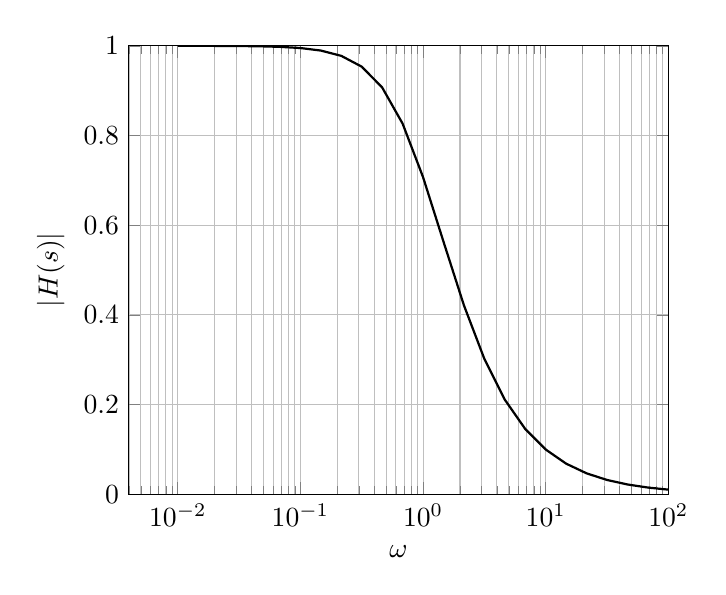
\begin{tikzpicture}
            \begin{semilogxaxis}[
                xlabel={$\omega$},
                ylabel={$|H(s)|$},
                grid=both,
                log basis x={10},
                xmax=100,
                domain=0.01:100,
                ymin=0,
                ymax=1
            ]
            
            \addplot[
                thick
            ]
            {1/sqrt(1 + x^2)};
            
            \end{semilogxaxis}
        \end{tikzpicture}
    \end{center}
    \caption{$|H(s)|$ vs. $\omega$ plot}
    \label{fig:butterworth lowpass plot}
\end{figure}
This is useful because it allows us 
to attenuate signals of high frequency, 
while allowing lower frequencies through 
unimpeded. This kind of circuit is 
known as a \emph{low-pass filter}, 
because low frequencies are allowed 
to pass. 

In this class, we are especially interested in 
the \emph{Butterworth} low-pass 
filter. For a general Butterworth
low-pass filter, 
\begin{equation} \label{eq:butterworth}
    \lvert H(j\omega) \rvert = \frac{\lvert K \rvert}{\sqrt{1 + \left( \frac{\omega}{\omega_c} \right)^{2n}}}
\end{equation}
where $n$ is the order of the 
filter, $K$ is a constant, and 
$\omega_c$ is the corner 
frequency, defined as the 
frequency at which the signal 
is $\frac{1}{\sqrt{2}}$ of 
the maximum value. In
the filter of figure \ref{fig:butterworth lowpass},
$n = 2$. In general, the 
larger the degree, the 
steeper the drop in 
$|H(s)|$.  
General Butterworth transfer
functions are known as 
\emph{normalized} Butterworth 
transfer functions, and 
are found by setting $\omega_c = 1$.
The normalized Butterworth 
transfer functions are listed in 
table \ref{tab:normalized butterworth}.

\subsection{Butterworth High-pass Filters}

A Butterworth high-pass filter does 
the opposite of a low-pass filter by 
letting high frequencies through 
and blocking low frequencies. To make 
a high-pass filter, simply interchange 
inductors and capacitors. Figure 
\ref{fig:butterworth highpass}
demonstrates a high-pass filter. 
\begin{figure}
    \begin{center}
        \begin{circuitikz}
            \draw (0,0) -- ++(-2,0)
            to[I, l=$i_{in}(t)$] ++(0,2)
            -- ++(2,0)
            to[R, l=$1\Omega$] ++(0,-2)
            -- ++(2,0)
            to[C, l=$1C$, v<=$v_v(t)$] ++(0,2)
            -- ++(-2,0);
        \end{circuitikz}
    \end{center}
    \caption{Butterworth high-pass filter}
    \label{fig:butterworth highpass}
\end{figure}
To spare the derivation, take it on 
faith that the transfer function 
for the filter in figure \ref{fig:butterworth highpass}
is 
\begin{equation}
    H(s) = \frac{s}{1+s}.
\end{equation}
Conversely from the low-pass filter, 
now $|H(s)|$ is near zero for 
small values of $s$ and near one 
for larger values.  

The steps to find a filter design 
for a specific need are as follows:
\begin{enumerate}
    \item Find filter order $n$
    \item Select corresponding 
    normalized transfer function 
    \item Reference the known 
    circuit configuration with 
    selected transfer function
    \item Find and adjust $\omega_c$ 
    if $A_{max} \neq 3dB$
    \item Scale magnitude and 
    frequency as necessary
\end{enumerate}
The filter order 
$n$ can be found by selecting 
the minimum integer $n$ such 
that 
\begin{equation}
    n \geq \frac{\log{\left( \frac{10^{0.1A_{min}} - 1}{10^{0.1A_{max}} - 1} \right)}}{2\log{(\frac{\omega_p}{\omega_s})}}
\end{equation}
where $\Omega_s = \frac{1}{\omega_s}$. 
A range of viable values for $\omega_c$
can by found with the formula given in 
eq. \ref{eq:omega scaling}
\begin{equation} \label{eq:omega scaling}
    \frac{1}{\left( 10^{0.1A_{max}} - 1 \right)^{\frac{1}{2n}}} \leq \omega_c \leq \frac{\frac{1}{\omega_s}}{\left( 10^{0.1A_{min}} - 1 \right)^{\frac{1}{2n}}}
\end{equation}
For high-pass filters, it's easier to 
find the right low-pass filter and 
then convert to a high-pass filter 
by changing all inductors to capacitors 
and vice versa. 
Let's do an example 
to illustrate.

Say we want a high-pass filter 
with the following specifications:
\begin{itemize}
    \item $A_{max} = 2dB$ ($H_{max} = -2dB$)
    \item $A_{min} = 40dB$ ($H_{min} = -40dB$)
    \item $\omega_s = 100Hz$
    \item $\omega_p = 1000Hz$. 
\end{itemize}
First, we need to find the 
minimum filter order. 
\begin{align}
    n &= \left\lceil \frac{\log{\left( \frac{10^{0.1A_{min}} - 1}{10^{0.1A_{max}} - 1} \right)}}{2\log{(\frac{\omega_p}{\omega_s})}} \right\rceil \\
    &= \left\lceil \frac{\log{\left( \frac{10^{0.1\times 40} - 1}{10^{0.1\times 2} - 1} \right)}}{2\log{(\frac{1000 Hz}{100 Hz})}} \right\rceil \\
    &= 3
\end{align}
Next, we take the corresponding transfer 
function from table \ref{tab:normalized butterworth}.
In this case it is 
\begin{equation}
    H(s) = \frac{1}{s^3 + 2s^2 + 2s + 1}.
\end{equation}
The circuit that goes with this transfer 
function is shown in figure \ref{tab:3rd order butterworth highpass}.
\begin{figure}
    \begin{center}
        \begin{circuitikz}
            \draw (0,0) -- ++(-2,0)
            to[V, l=$v_{IN}(t)$] ++(0,2)
            to[R, l=$R_s$] ++(2,0)
            to[C, l=$C_1$] ++(0,-2)
            -- ++(2,0)
            to[C, l=$C_2$, v<=$v_{out}(t)$] ++(0,2)
            to[L, l=$L$] ++(-2,0);
        \end{circuitikz}
    \end{center}
    \caption{3rd order high-pass filter}
    \label{fig:3rd order butterworth highpass}
\end{figure}
\begin{align}
    H(s) &= \frac{V_{out}(s)}{V_{in}(s)} \\
    &= \frac{1}{s^3R_sLC_1C_2 + s^2LC_2 + sR_s(C_1+C_2) + 1} \\
    &= \frac{1}{s^3 + 2s^2 + 2s + 1} \\
    R_sLC_1C_2 &= 1 \\
    LC_2 &= 2 \\
    R_s(C_1 + C_2) &= 2 \\
    R_s &= 1 \\
    C_1 &= 0.5 \\
    C_2 &= 1.5 \\
    L &= \frac{4}{3}
\end{align}
We now need to adjust $\omega_c$, 
since $\omega_c \neq \omega_p$. 
To do this, we can get 
a range of values that would 
work using the formula in 
eq. \ref{eq:omega scaling}.
We find that 
\begin{equation}
    \omega_c \in \left[ 1.094, 2.15 \right]
\end{equation}
Whatever value of $C_1$, $C_2$, and $L$ 
we choose, we would need to scale 
each by $\frac{1}{\omega_c}$. 
We would then substitute these 
values into our circuit, 
and our high-pass filter is 
complete.

\subsection{Active Low-pass Filters}

So far every low-pass filter 
we have seen requires an 
inductor. This is problematic 
once you recall that 
inductors are the most 
non-ideal element we have 
seen to date. We can craft 
a better low-pass filter 
by using op-amps and
avoiding inductors. Figure 
\ref{fig:op-amp low-pass filter}
demonstrates the simplest 
low-pass filter using an op-amp, 
called an \emph{active} filter 
as opposed to the \emph{passive}
inductor-based low-pass 
filter. 
\begin{figure}
    \begin{center}
        \begin{circuitikz}[european resistors]
            \draw (0, 0) node[op amp] (opamp) {};
            \draw (opamp.-)to[R, -o, l=$Z_{IN}$] ++(-2,0)
            node[left] {$v_{IN}(t)$};
            \draw (opamp.-) -- ++(-0.1  ,0)
            -- ++(0,1)
            to[R, l=$Z_F$] ++(2.5,0)
            to[short] (opamp.out)
            to[short, -o] ++(0.25,0)
            node[right] {$v_{OUT}(t)$};
            \draw (opamp.+) -- ++(0,-1)
            node[ground] {};
        \end{circuitikz}
    \end{center}
    \caption{Active low-pass filter}
    \label{fig:op-amp low-pass filter}
\end{figure}
The transfer function can be quickly calculated as 
\begin{align}
    H(s) &= \frac{V_{out}(s)}{V_{in}(s)} \\
    &= -\frac{Z_F(s)}{Z_{in}(s)}.
\end{align}
Let's see how we can construct 
a circuit whose transfer 
function is identical to the 
normalized first order 
Butterworth transfer function, 
\begin{equation}
    H(s) = \frac{1}{s+1}.
\end{equation}
Since we know that, for 
the circuit in figure 
\ref{fig:op-amp low-pass filter}
$H(s) = -\frac{Z_F(s)}{Z_{in}(s)}$, 
an appropriate configuration
could be that of figure 
\ref{fig:op-amp low-pass filter with parallel RC}.
\begin{figure}
    \begin{center}
        \begin{circuitikz}
            \draw (0, 0) node[op amp] (opamp) {};
            \draw (opamp.-)to[R, -o, l=$1\Omega$] ++(-2,0)
            node[left] {$v_{IN}(t)$};
            \draw (opamp.-) -- ++(-0.1,0)
            -- ++(0,1)
            to[short] ++(0.5,0) coordinate (A)
            to[R, l=$1\Omega$] ++(2,0) 

            (A) to[short] ++(0,1.5) coordinate (B)
            (B) to[C, l=$1F$] ++(2,0) coordinate (C)
            (C) to[short] ++(0,-1.5)
            -- (opamp.out)
            to[short, -o] ++(0.25,0) node[right] {$v_{OUT}(t)$};
            
            \draw (opamp.+) -- ++(0,-1)
            node[ground] {};
        \end{circuitikz}
    \end{center}
    \caption{Active low-pass filter}
    \label{fig:op-amp low-pass filter with parallel RC}
\end{figure}
We see that $Z_F = \frac{1}{s + 1}$, while $Z_{IN} = 1$. 
Thus
\begin{align}
    H(s) &= -\frac{Z_F(s)}{Z_{in}(s)} \\
    &= -\frac{\frac{1}{s + 1}}{1} \\
    &= -\frac{1}{s + 1}.
\end{align}
We can construct higher-order 
filters by chaining first-order 
filters together. Consider 
figure \ref{fig:chained op-amp low-pass filters}.
\begin{figure}
    \begin{center}
        \begin{circuitikz}[european resistors]
            \draw (0, 0) node[op amp] (opamp) {};
            \draw (opamp.-) to[R, -o, l=$Z_{IN1}$] ++(-2,0)
            node[left] {$v_{IN}(t)$};
            \draw (opamp.-) -- ++(-0.1  ,0)
            -- ++(0,1)
            to[R, l=$Z_{F1}$] ++(2.5,0)
            to[short] (opamp.out)
            to[short, -o] ++(0.25,0) coordinate (A);
            \draw (opamp.+) -- ++(0,-1)
            node[ground] {};

            \draw (4.5, -0.5) node[op amp] (opamp) {};
            \draw (opamp.-) to[R, -o, l=$Z_{IN2}$] (A);
            \draw (opamp.-) -- ++(-0.1  ,0)
            -- ++(0,1)
            to[R, l=$Z_{F2}$] ++(2.5,0)
            to[short] (opamp.out)
            to[short, -o] ++(0.25,0)
            node[right] {$v_{OUT}(t)$} coordinate (A);
            \draw (opamp.+) -- ++(0,-1)
            node[ground] {};
        \end{circuitikz}
    \end{center}
    \caption{Chained active low-pass filters}
    \label{fig:chained op-amp low-pass filters}
\end{figure}
With a bit of calculation, we 
can show that 
\begin{align}
    H(s) &= \frac{V_{OUT}(s)}{V_{IN}(s)} \\
    &= \frac{-V_{OUT1}(s) \frac{-Z_{F2}(s)}{Z_{IN2}(s)}}{V_{IN}(s)} \\
    &= \frac{-\left(-V_{IN}(s)\frac{Z_{F1}}{Z_{IN1}}\right) \frac{-Z_{F2}(s)}{Z_{IN2}(s)}}{V_{IN}(s)} \\
    &= \frac{Z_{F1}(s)}{Z_{IN1}(s)} \frac{Z_{F2}(s)}{Z_{IN2}(s)}
\end{align}
We can construct up to a second 
degree polynomial in the numerator 
and up to a second degree polynomial 
in the denominator using parallel 
combinators of capacitors and 
resistors. By chaining $n$ op-amps, 
we can make the $n$th Butterworth 
transfer function. With 
magnitude and frequency 
scaling, we can make any 
$n$th degree transfer function, 
with a small caveat. The caveat is 
that the poles will only be real, 
assuming we use only capacitors and 
resistors. If we introduce 
indcuctors then we can encounter 
filters with complex poles, but 
avoiding inductors is the entire 
reason we made active op-amps. We
find a solution to this conundrum
with a different filter topology. 
Figure \ref{fig:sallen and key}
demonstrates one possible 
configuration, called 
a Sallen and Key filter. 
\begin{figure}
    \begin{center}
        \begin{circuitikz}
            \draw (0, 0) node[op amp] (opamp) {};

            \draw (opamp.+) -- ++(-1,0) coordinate (A)
            to[C, l=$C_2$] ++(0,1)
            -- ++(-2,0)
            node[ground] {}
            (A) to[R, l=$R_2$] ++(-2,0) coordinate (B)
            to[R, -o, l=$R_1$] ++(-2,0)
            node[left] {$v_{IN}(t)$}
            (B) -- ++(0,-2)
            to[C, l=$C_1$] ++(5.365,0)
            -- (opamp.out)
            to[short, -o] ++(1,0)
            node[right] {$v_{OUT}(t)$}
            (opamp.-) -- ++(0,1) coordinate (C)
            to[R, l=$R_B$] ++(0,2)
            -- ++(-1,0)
            node[ground] {}
            (C) to[R, l=$R_A$] ++(2.39,0)
            -- (opamp.out);
        \end{circuitikz}
    \end{center}
    \caption{Sallen and Key filter}
    \label{fig:sallen and key}
\end{figure}
With a lot of elbow grease, 
the transfer function 
for the Sallen and Key 
filter can be shown to 
be 
\begin{equation} \label{eq:sallen and key}
    H(s) = \frac{ \frac{ 1 + \frac{R_A}{R_B} }{R_1R_2C_1C_2} }{ s^2 + \left( \frac{1}{R_1C_1} + \frac{1}{R_2C_1} - \frac{R_A}{R_BR_2C_2} \right)s + \frac{1}{R_1R_2C_1C_2} }
\end{equation}
This unwieldy beast can 
be simplified if we let 
$R_A = 0$ and $R_B = \infty$. 
This configuration
corresponds to figure 
\ref{fig:simple sallen and key}.
\begin{figure}
    \begin{center}
        \begin{circuitikz}
            \draw (0, 0) node[op amp] (opamp) {};

            \draw (opamp.+) -- ++(-1,0) coordinate (A)
            to[C, l=$C_2$] ++(0,1)
            -- ++(-2,0)
            node[ground] {}
            (A) to[R, l=$R_2$] ++(-2,0) coordinate (B)
            to[R, -o, l=$R_1$] ++(-2,0)
            node[left] {$v_{IN}(t)$}
            (B) -- ++(0,-2)
            to[C, l=$C_1$] ++(5.365,0)
            -- (opamp.out)
            to[short, -o] ++(1,0)
            node[right] {$v_{OUT}(t)$}
            (opamp.-) -- ++(0,1)
            -- ++(2.39,0)
            -- (opamp.out);
        \end{circuitikz}
    \end{center}
    \caption{Simplified Sallen and Key filter}
    \label{fig:simple sallen and key}
\end{figure}
Eq. \ref{eq:sallen and key}
simplifies to 
\begin{equation} \ref{eq:sallen and key transfer}
    H(s) = \frac{ \frac{1}{R_1R_2C_1C_2} }{ s^2 + \left( \frac{1}{(R_1||R_2)C_1} \right)s + \frac{1}{R_1R_2C_1C_2} }
\end{equation}
We can express this 
as 
\begin{equation}
    H(s) = \frac{K_0}{s^2 + 2\sigma s + \omega^2_0}
\end{equation}
where 
\begin{align}
    2\sigma &= \frac{1}{(R_1 || R_2)C_1}, \\
    \omega_0 &= \sqrt{ \frac{1}{R_1R_2C_1C_2} },
\end{align}
and 
\begin{equation}
    K_0 = \frac{1}{R_1R_2C_1C_2}
\end{equation}

Let's bring this all 
together with an example. 
Say we wish to find the circuit 
whose transfer function is 
\begin{align} \label{eq:example transfer}
    H(s) &= \frac{1}{s^3 + 2s^2 + 2s + 1} \\
    &= \frac{1}{(s+1)(s^2+s+1)} \\
    &= -\left( -\frac{1}{s+1} \right)\left( \frac{1}{s^2+s+1} \right)
\end{align}
We already know how to make
the filter whose transfer function 
is $-\frac{1}{s+1}$, and for 
the negative in front we 
just need an inverting 
op-amp with gain of $1$. 
That leaves us to find 
the circuit whose transfer 
function is 
\begin{equation} \label{eq:example sallen and key transfer}
    \frac{1}{s^2+s+1}.
\end{equation} 
Since the roots are complex, 
we know we'll need a Sallen 
and Key filter. If we compare 
the form of eq. \ref{eq: example sallen and key transfer}
to eq. \ref{eq:sallen and key transfer}, 
we see that we need 
\begin{align}
    \frac{1}{(R_1||R_2)C_1} &= 1 \\
    \frac{1}{R_1R_2C_1C_2} &= 1.
\end{align}
Since we have two equations but 
four unknowns, there will be 
an infinite number of 
solutions for our elements. 
Let's choose 
\begin{align}
    R_1 &= 1\Omega \\
    R_2 &= 1\Omega \\
    C_1 &= 2F \\
    C_2 &= 0.5F
\end{align}
Then the circuit whose transfer 
function is eq. \ref{eq:example transfer}
is shown in figure \ref{fig:example solution}.
\begin{figure}
    \begin{center}
        \begin{circuitikz}
            \draw (0, 0) node[op amp] (opamp) {};
            \draw (opamp.out) -- ++(0,2)
            to[R, l=$10k\Omega$] ++(-2.375,0)
            -- (opamp.-)
            to[R, -o, l=$10k\Omega$] ++(-1.5,0)
            node[left] {$v_{IN}(t)$}
            (opamp.+) node[ground] {};

            \draw (4, -0.5) node[op amp] (op-amp) {};
            \draw (op-amp.+) node[ground] {}
            (op-amp.-) to[R, l=$1\Omega$] (opamp.out)
            (op-amp.-) -- ++(0,1) coordinate (Z)
            to[R, l=$1\Omega$] ++(2.4,0) coordinate (Y)
            -- (op-amp.out)
            (Z) -- ++(0,1.5)
            to[C, l=$1F$] ++(2.4,0)
            -- (Y);

            \draw (12, 0) node[op amp] (opamp) {};
            \draw (opamp.+) -- ++(-1,0) coordinate (A)
            to[C, l=$0.5 F$] ++(0,1)
            -- ++(-2,0)
            node[ground] {}
            (A) to[R, l=$1\Omega$] ++(-2,0) coordinate (B)
            to[R, l=$1\Omega$] ++(-2,0)
            -- (op-amp.out)
            (B) -- ++(0,-2)
            to[C, l=$2F$] ++(5.365,0)
            -- (opamp.out)
            to[short, -o] ++(1,0)
            node[right] {$v_{OUT}(t)$}
            (opamp.-) -- ++(0,1)
            -- ++(2.39,0)
            -- (opamp.out);
        \end{circuitikz}
    \end{center}
    \caption{Complete topology}
    \label{fig:example solution}
\end{figure}

\newpage

\subsection{Reference}

\begin{figure}
    \begin{center}
        \begin{tabular}{c | c | c }
            & Parallel & Series \\
            \hline
            $B_{\omega}$ & $\frac{1}{RC}$ & $\frac{R}{L}$ \\
            $Q$ & $R\sqrt{\frac{C}{L}}$ & $\frac{1}{R}\sqrt{\frac{L}{C}}$ \\
        \end{tabular}
    \end{center}
    \caption{RLC response parameters}
    \label{tab:RLC response parameters}
\end{figure}

\begin{align}
    H_{RLC}(s) &= \frac{\frac{s}{C}}{s^2 + \frac{s}{RC} + \frac{1}{LC}} \\
    &= \frac{\frac{s}{C}}{s^2 + \frac{\omega_m s}{Q} + \omega^2_r}
\end{align}

\begin{figure}
    \begin{center}
        \begin{tabular}{c | c}
            $n$ & $H(s)$ \\
            \hline
            $1$ & $\frac{1}{s+1}$ \\
            $2$ & $\frac{1}{s^2+\sqrt{2}s + 1}$ \\
            $3$ & $\frac{1}{s^3 + 2s^2 + 2s + 1}$ \\
            $4$ & $\frac{1}{(s^{2}+\sqrt{2-\sqrt{2} } s+1)(s^{2}+\sqrt{2+\sqrt{2} } s+1)}$ \\
            $5$ & $\frac{1}{(s+1)(s^2+\phi^{-1} s+1)(s^2+\phi s+1)}$
        \end{tabular}
    \end{center}
    \caption{Normalized Butterworth transfer functions}
    \label{tab:normalized butterworth}
\end{figure}

\pagebreak

\section{Conclusion}

We have arrived at the end now. 
You will take your final exams 
and eventually forget the 
majority of what you learned
here. What will remain after 
five months, five years, time 
so precious but so abstract, 
will be your curiousity, the 
methods by which you explore the 
world, and the knowledge that 
you applied yourself, did your 
best, and grew. Do not waste 
the opportunity that living 
affords you. Do not content 
yourself with mere existence. 
Hunger for growth, \emph{starve}
for it. Move ever forward
and remember that 
one day you may no more 
remember the experiences you 
have had than the meals you have 
eaten, but even so they have 
made you.

\end{document}
